\chapter[APLICACIONES DEL ÁLGEBRA LINEAL]{APLICACIONES DEL \\ ÁLGEBRA LINEAL}
\printchaptertableofcontents

Este capítulo consta de 10 aplicaciones del álgebra lineal. Cada aplicación se encuentra en su propia sección independiente, por lo que las secciones se pueden eliminar o permutar según se desee. Dado que nuestro objetivo principal en este capítulo es presentar aplicaciones del álgebra lineal, omitiremos algunas demostraciones. Siempre que se necesiten resultados de otros campos, se enunciaran de manera precisa, con motivación cuando sea posible, pero generalmente sin demostración.

\section{Interpolación mediante splines cúbicos}

Ajustar una curva a través de puntos específicos en el plano es un problema común que se encuentra en el análisis de datos experimentales, en la determinación de las relaciones entre las variables y en el trabajo de diseño. Una aplicación omnipresente está en el diseño y la descripción de las fuentes de ordenador e impresora, como las fuentes PostScript\texttrademark ~y TrueType\texttrademark.
\begin{figure}[h!]
    \centering
    
\includegraphics[width=0.3\textwidth]{Images/Capitulo8/R.pdf}
    \caption{La ‘R’ en PostScript\texttrademark ~y TrueType\texttrademark}
\end{figure}

\newpage

En la figura \ref{fig:inter1} se muestran siete puntos en el plano $xy$, y en la figura \ref{fig:inter3} se ha dibujado una curva suave que pasa a través de ellos. Se dice que una curva que pasa a través de un conjunto de puntos en el plano \emph{interpola} esos puntos, y la curva se llama \emph{curva de interpolación} para esos puntos. La curva de interpolación de la figura \ref{fig:inter3} se dibujó con la ayuda de un spline de dibujo (figura \ref{fig:inter2}). Esta ayuda de dibujo consiste en una tira delgada y flexible de madera u otro material que se dobla para pasar a través de los puntos que se van a interpolar. Los pesos deslizantes adjuntos mantienen la spline en posición mientras el artista dibuja la curva de interpolación. La spline de dibujo servirá como modelo físico para una teoría matemática de la interpolación que discutiremos en esta sección.
\begin{figure*}[h!]
    \centering
    \subfloat[\label{fig:inter1}]{
    \begin{tikzpicture}[scale=1.4]
        \draw[-Stealth,thick] (-0.15,0) -- (3,0) node[above left, yshift=2pt] {$x$};
        \draw[-Stealth,thick] (0,-0.15) -- (0,2) node[below right, xshift=2pt] {$y$};
        \filldraw (0.5,{0.5*(0.5 - 2)^3 + (0.5 - 2)^2 + 0.5}) circle (1.5pt);
        \filldraw (0.9,{0.5*(0.9 - 2)^3 + (0.9 - 2)^2 + 0.5}) circle (1.5pt);
        \filldraw (1.3,{0.5*(1.3 - 2)^3 + (1.3 - 2)^2 + 0.5}) circle (1.5pt);
        \filldraw (1.7,{0.5*(1.7 - 2)^3 + (1.7 - 2)^2 + 0.5}) circle (1.5pt);
        \filldraw (2.1,{0.5*(2.1 - 2)^3 + (2.1 - 2)^2 + 0.5}) circle (1.5pt);
        \filldraw (2.5,{0.5*(2.5 - 2)^3 + (2.5 - 2)^2 + 0.5}) circle (1.5pt);
        \filldraw (2.8,{0.5*(2.8 - 2)^3 + (2.8 - 2)^2 + 0.5}) circle (1.5pt);
    \end{tikzpicture}
    } \hfill
    \subfloat[\label{fig:inter2}]{
    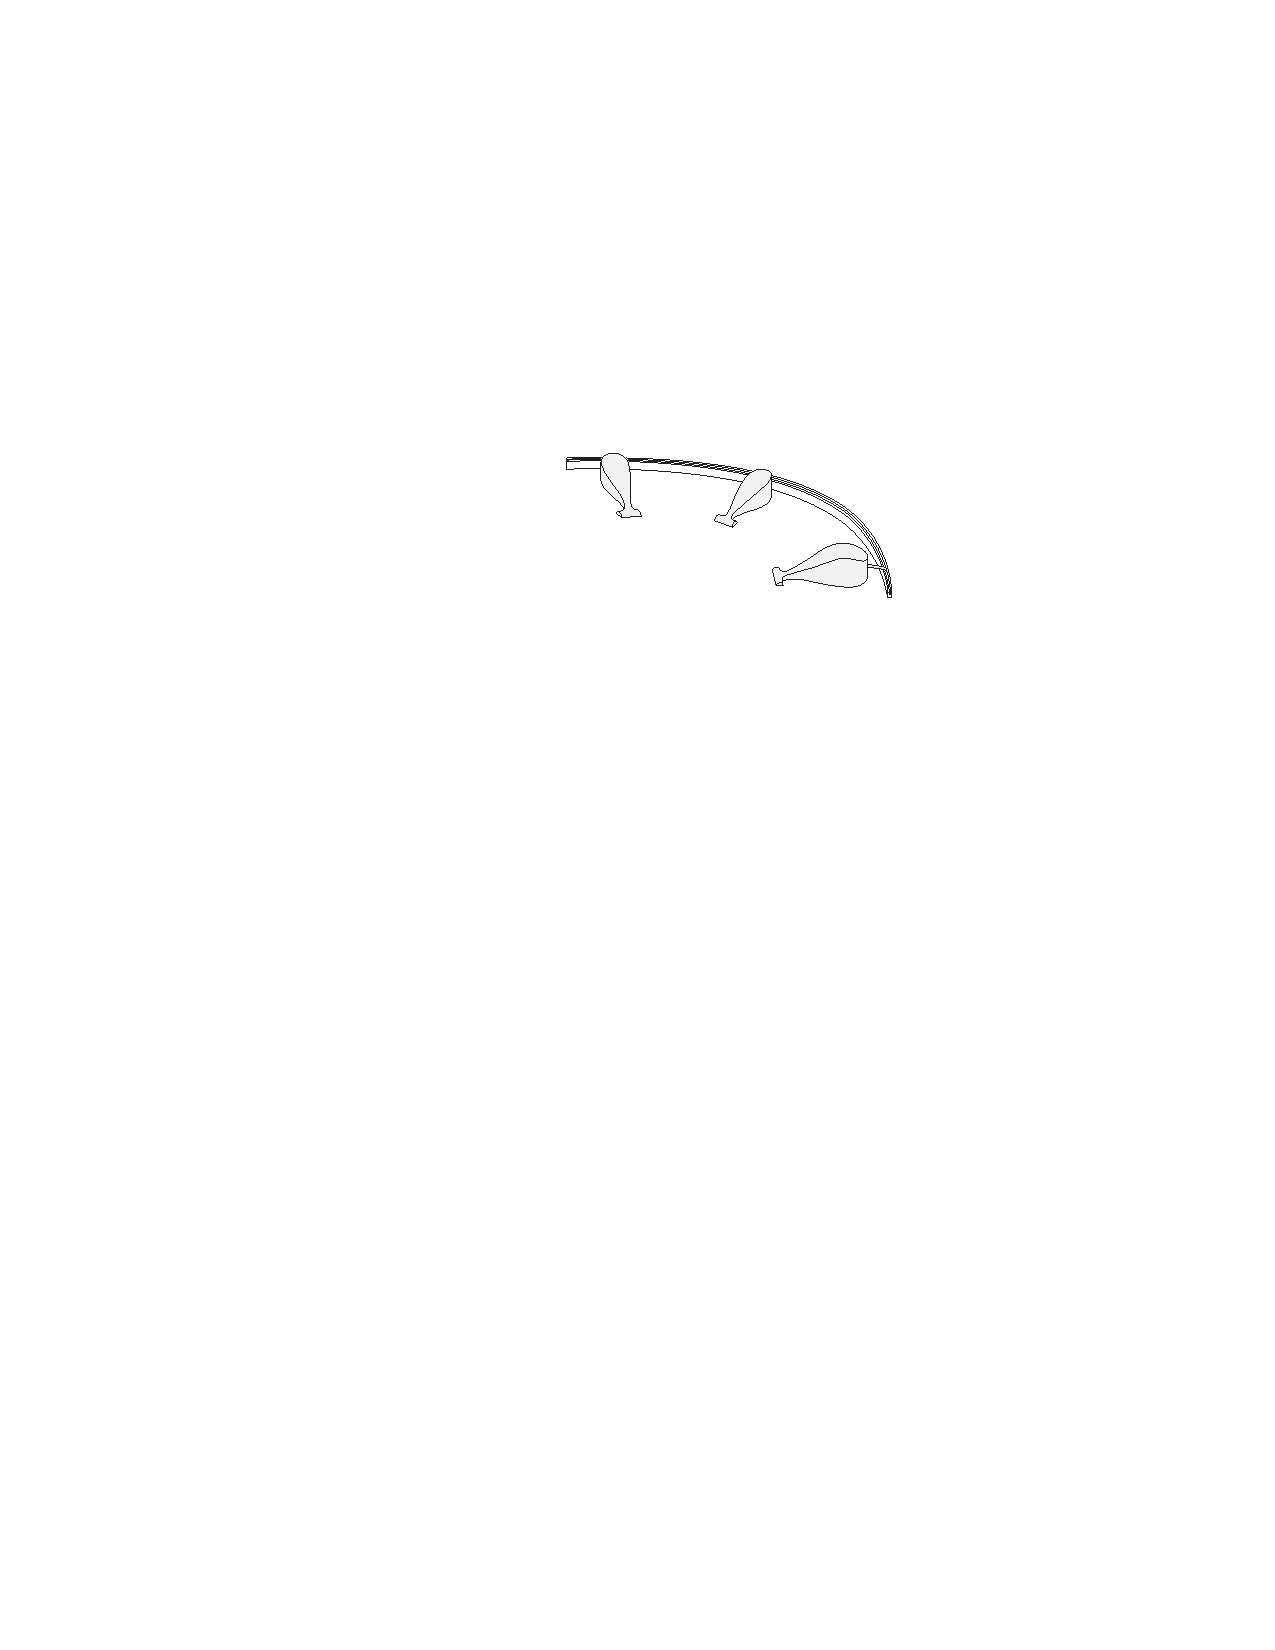
\includegraphics[height=3cm]{Images/Capitulo8/drafting_spline.pdf}
    } \hfill
    \subfloat[\label{fig:inter3}]{
    \begin{tikzpicture}[scale=1.4]
        \draw[-Stealth,thick] (-0.15,0) -- (3,0) node[above left, yshift=2pt] {$x$};
        \draw[-Stealth,thick] (0,-0.15) -- (0,2) node[below right, xshift=2pt] {$y$};
        \draw[gray, domain=0.25:2.9, samples=100] plot(\x,{0.5*(\x - 2)^3 + (\x - 2)^2 + 0.5});
        \filldraw (0.5,{0.5*(0.5 - 2)^3 + (0.5 - 2)^2 + 0.5}) circle (1.5pt);
        \filldraw (0.9,{0.5*(0.9 - 2)^3 + (0.9 - 2)^2 + 0.5}) circle (1.5pt);
        \filldraw (1.3,{0.5*(1.3 - 2)^3 + (1.3 - 2)^2 + 0.5}) circle (1.5pt);
        \filldraw (1.7,{0.5*(1.7 - 2)^3 + (1.7 - 2)^2 + 0.5}) circle (1.5pt);
        \filldraw (2.1,{0.5*(2.1 - 2)^3 + (2.1 - 2)^2 + 0.5}) circle (1.5pt);
        \filldraw (2.5,{0.5*(2.5 - 2)^3 + (2.5 - 2)^2 + 0.5}) circle (1.5pt);
        \filldraw (2.8,{0.5*(2.8 - 2)^3 + (2.8 - 2)^2 + 0.5}) circle (1.5pt);
    \end{tikzpicture}
    }
    \caption{Ejemplos de curvas interpolación}
    \label{fig:enter-label}
\end{figure*}

\section*{Ajuste de curva}

Supongamos que se nos dan $n$ puntos en el plano $xy$,
$$(x_1, y_1), (x_2, y_2), \dots, (x_n, y_n)$$
que deseamos interpolar con una curva “bien comportada” (figura \ref{fig:bienc}). Para mayor comodidad, tomamos los puntos equiespaciados en la dirección $x$, aunque nuestros resultados se pueden extender fácilmente al caso de puntos desigualmente espaciados. Si tomamos la distancia común entre las coordenadas $x$ de los puntos como $h$, entonces tenemos
$$x_2-x_1=x_3-x_2=\cdots=x_n-x_{n-1}=h$$
Sea $y = S(x)$, $x_1 \leq x \leq x_n$, la curva interpolante que buscamos. Suponemos que esta curva describe el desplazamiento de una regla flexible que interpola los $n$ puntos cuando los pesos que sujetan la regla se sitúan precisamente en los $n$ puntos.
\begin{figure}[h!]
    \centering
    \begin{tikzpicture}[
        declare function={
        f(\x) = 0.0125*\x^4 - 0.15*\x^3 + 0.3625*\x^2 + 0.525*\x + 1;
        x1=0;
        x2=1;
        x3=2;
        x4=3;
        x5=4;
        x6=5;
        x7=6;
        }]
        \draw[-Stealth,thick] (-0.15,0) -- (9.25,0) node[above left, yshift=2pt] {$x$};
        \draw[-Stealth,thick] (0,-0.15) -- (0,4) node[below right, xshift=2pt] {$y$};
        \begin{scope}[xshift=1.5cm]
            \draw[gray, domain=0:6, samples=100] plot(\x,{f(\x)});
            \foreach \i in {1,2,3,...,7}
            \filldraw (x\i,{f(x\i)}) circle (1.5pt);
            \foreach \j in {1,2,3,5,6,7}
            \draw[dash pattern=on 3pt off 3pt] (x\j,{f(x\j)}) -- (x\j,0);
            \node at (x7,{f(x7)}) [right] {$(x_n, y_n)$};
            \node at (x6,{f(x6)}) [right] {$(x_{n-1}, y_{n-1})$};
            \node at (x1,{f(x1)}) [left] {$(x_1, y_1)$};
            \node at (x2,{f(x2)}) [left] {$(x_2, y_2)$};
            \node at (x3,{f(x3)}) [left] {$(x_3, y_3)$};
            \foreach \k in {1,2,5,6} {
            \draw[latex-latex] (x\k,0.4) -- (x{\k+1},0.4);
            \node[fill=white,minimum size=0.1mm] at ({0.5*(x\k+x\k+1)},0.4) {$h$};
            }
            \draw[latex-] (3.6,{f(3.6) + 0.05}) -- (4,{f(4) + 0.75}) node[right] {$y = S(x)$};
            \node at (x4,0.4) {$\cdots$};
        \end{scope}
    \end{tikzpicture}
    \caption{~}
    \label{fig:bienc}
\end{figure}

Se sabe, por la teoría de vigas lineales, que para pequeños desplazamientos, la cuarta derivada del desplazamiento de una viga es cero a lo largo de cualquier intervalo del eje $x$ que no contenga fuerzas externas actuando sobre la viga. Si tratamos nuestra regla flexible como una viga delgada y comprendemos que las únicas fuerzas externas actuando sobre ella provienen de los pesos en los $n$ puntos especificados, entonces se sigue que
$$S^{(4)}(x) \equiv 0$$
para valores de $x$ que se encuentran en los $n-1$ intervalos abiertos
$$(x_1, x_2), (x_2, x_3), \dots , (x_{n-1}, x_n)$$
entre los $n$ puntos.

También necesitamos el resultado de la teoría de vigas lineales que establece que, para una viga sujeta únicamente a fuerzas externas, el desplazamiento debe tener dos derivadas continuas. En el caso de la curva interpolante $y = S(x)$ construida con la regla flexible, esto significa que $S(x)$, $S′(x)$ y $S′′(x)$ deben ser continuas para $x_1 \leq x \leq x_n$.

La condición de que $S′′(x)$ sea continua es lo que hace que una regla flexible produzca una curva agradable, ya que resulta en una curvatura continua. El ojo puede percibir cambios bruscos en la curvatura, es decir, discontinuidades en $S′′(x)$, pero los cambios bruscos en derivadas de orden superior no son discernibles. Por lo tanto, la condición de que $S′′(x)$ sea continua es el requisito mínimo para que la curva interpolante sea perceptible como una curva suave única, en lugar de una serie de curvas separadas unidas.

Para determinar la forma matemática de la función $S(x)$, observamos que, dado que $S^{(4)}(x) \equiv 0$ en los intervalos entre los $n$ puntos especificados, se sigue que al resolver esta ecuación repetidamente, $S(x)$ debe ser un polinomio cúbico en $x$ en cada uno de esos intervalos. Sin embargo, en general, $S(x)$ será un polinomio cúbico diferente en cada intervalo, por lo que $S(x)$ debe tener la forma
\begin{equation}
    S(x) = \begin{cases}
        \begin{aligned}
            & S_1(x), & x_1 & \leq x \leq x_2 \\
            & S_2(x), & x_2 & \leq x \leq x_3 \\
            & \phantom{SS} \vdots & & \;\quad \vdots \\
            & S_{n-1}(x), & x_{n-1} & \leq x \leq x_n
        \end{aligned}
    \end{cases} \label{eq:S_interpola}
\end{equation}
donde $S_1(x)$, $S_2(x)$, $\dots$, $S_{n-1}(x)$ son polinomios cúbicos. Para mayor comodidad, los escribiremos de la forma
\begin{align*}
    S_1(x) & = a_1(x - x_1)^3 + b_1(x - x_1)^2 + c_1(x - x_1) + d_1, & x_1 & \leq x \leq x_2 \\
    S_2(x) & = a_2(x - x_2)^3 + b_2(x - x_2)^2 + c_2(x - x_2) + d_2, & x_2 & \leq x \leq x_3 \\
    & \vdots & & \\
    S_{n-1}(x) & = a_{n-1}(x - x_{n-1})^3 + b_{n-1}(x - x_{n-1})^2 & & \\
    & \hspace{3.25cm} + c_{n-1}(x - x_{n-1}) + d_{n-1}, & x_{n-1} & \leq x \leq x_n
\end{align*}
Los $a_i$, $b_i$, $c_i$ y $d_i$ constituyen un total de $4n - 4$ coeficientes que debemos determinar para especificar completamente $S(x)$. Si elegimos estos coeficientes de manera que $S(x)$ interpole los $n$ puntos especificados en el plano y que $S(x)$, $S'(x)$ y $S''(x)$ sean continuos, entonces la curva interpolante resultante se llama \emph{spline cúbico}.

Primero, derivando la expresión \eqref{eq:S_interpola}, es decir, derivando cada polinomio anterior, se sigue que
\begin{align*}
    S'_1(x) & = 3a_1(x - x_1)^2 + 2b_1(x - x_1) + c_1, & x_1 & \leq x \leq x_2 \\
    S'_2(x) & = 3a_2(x - x_2)^2 + 2b_2(x - x_2) + c_2, & x_2 & \leq x \leq x_3 \\
    & \vdots & & \\
    S'_{n-1}(x) & = 3a_{n-1}(x - x_{n-1})^2 + 2b_{n-1}(x - x_{n-1}) + c_{n-1}, & x_{n-1} & \leq x \leq x_n
\end{align*}\newpage\noindent
y derivando nuevamente, obtenemos que
\begin{align*}
    S''_1(x) & = 6a_1(x - x_1) + 2b_1, & x_1 & \leq x \leq x_2 \\
    S''_2(x) & = 6a_2(x - x_2) + 2b_2, & x_2 & \leq x \leq x_3 \\
    & \vdots & & \\
    S''_{n-1}(x) & = 6a_{n-1}(x - x_{n-1}) + 2b_{n-1}, & x_{n-1} & \leq x \leq x_n
\end{align*}
Ahora utilizaremos estas ecuaciones y las cuatro propiedades de los splines cúbicos que se indican a continuación para expresar los coeficientes desconocidos $a_i$, $b_i$, $c_i$, $d_i$ con $i = 1, 2, \dots, n - 1$, en términos de las coordenadas conocidas $y_1$, $y_2$, $\dots$, $y_n$.

\begin{tcolorbox}[
        arc=0mm, 
        bottomtitle=0.5mm,
        boxrule=0mm,
        colbacktitle=black!10!white, 
        coltitle=black,
        left=2.5mm,
        leftrule=1mm,
        right=3.5mm,
        title={$S(x)$ interpola los puntos $(x_i, y_i)$ con $i = 1, 2, \dots, n$.},
        toptitle=0.75mm,
        colframe=black!30!white,
    ]
    Debido a que $S(x)$ interpola los puntos $(x_i, y_i)$, con $i = 1, 2, \dots, n$, tenemos
    \begin{equation}
        S(x_1) = y_1, S(x_2) = y_2, \dots, S(x_n) = y_n \label{YQUJAJAJAJAJJA}
    \end{equation}
    De las primera $n - 1$ de estas ecuaciones y \eqref{eq:S_interpola}, obtenemos
    \begin{equation}
        d_1 = y_1, d_2 = y_2, \dots, d_{n-1} = y_{n-1} \label{UAJAJJAUAUHVCFATQHH}
    \end{equation}
    De la última ecuación en \eqref{YQUJAJAJAJAJJA}, la última ecuación en \eqref{eq:S_interpola}, y el hecho de que $x_n - x_{n-1} = h$, obtenemos
    \begin{equation}
        a_{n-1}h^3 + b_{n-1}h^2 + c_{n-1}h + d_{n-1} = y_n \label{UAJAJAHHCCFGYYQUYQHUU}
    \end{equation}
\end{tcolorbox}

\begin{tcolorbox}[
        arc=0mm, 
        bottomtitle=0.5mm,
        boxrule=0mm,
        colbacktitle=black!10!white, 
        coltitle=black,
        left=2.5mm,
        leftrule=1mm,
        right=3.5mm,
        title={$S(x)$ es continua en $[x_1, x_n]$.},
        toptitle=0.75mm,
        colframe=black!30!white,
    ]
    Debido a que $S(x)$ es continuo para $x_1 \leq x \leq x_n$, se deduce que en cada punto $x_i$ en el conjunto $x_2$, $x_3$, $\dots$, $x_{n-1}$ debemos tener
    \begin{equation}
        S_{i-1}(x_i) = S_i(x_i), \quad i = 2, 3, \dots, n-1 \label{JAJAJAJJAJAVHHGGGQ}
    \end{equation}
    De lo contrario, las gráficas de $S_{i-1}(x)$ y $S_i(x)$ no se unirían para formar una curva continua en $x_i$. Cuando aplicamos la propiedad de interpolación $S_i(x_i) = y_i$, se sigue de \eqref{JAJAJAJJAJAVHHGGGQ} que $S_{i-1}(x_i) = y_i$ donde $i = 2, 3, \dots, n-1$, o de \eqref{eq:S_interpola} que
    \begin{equation}
        \begin{aligned}
            a_1h^3 + b_1h^2 + c_1h + d_1 & = y_2 \\
            a_2h^3 + b_2h^2 + c_2h + d_2 & = y_3 \\
            & \vdots \\
            a_{n-2}h^3 + b_{n-2}h^2 + c_{n-2}h + d_{n-2} & = y_{n-1}
        \end{aligned} \label{UAUAJAHCCGTTQRTQHCCTAT}
    \end{equation}
\end{tcolorbox}

\begin{tcolorbox}[
        arc=0mm, 
        bottomtitle=0.5mm,
        boxrule=0mm,
        colbacktitle=black!10!white, 
        coltitle=black,
        left=2.5mm,
        leftrule=1mm,
        right=3.5mm,
        title={$S'(x)$ es continua en $[x_1, x_n]$.},
        toptitle=0.75mm,
        colframe=black!30!white,
    ]
    Debido a que $S'(x)$ es continuo para $x_1 \leq x \leq x_n$, se deduce que
    $$S'_{i-1}(x_i) = S'_i(x_i), \quad i = 2, 3, \dots, n-1$$
    es decir
    \begin{equation}
        \begin{aligned}
            3a_1h^2 + 2b_1h + c_1 & = c_2 \\
            3a_2h^2 + 2b_2h + c_2 & = c_3 \\
            & \vdots \\
            3a_{n-2}h^2 + 2b_{n-2}h + c_{n-2} & = c_{n-1}
        \end{aligned} \label{HAJAHAHCCFGYYYAGQTTQYQHHA}
    \end{equation}
\end{tcolorbox}

\newpage

\begin{tcolorbox}[
        arc=0mm, 
        bottomtitle=0.5mm,
        boxrule=0mm,
        colbacktitle=black!10!white, 
        coltitle=black,
        left=2.5mm,
        leftrule=1mm,
        right=3.5mm,
        title={$S''(x)$ es continua en $[x_1, x_n]$.},
        toptitle=0.75mm,
        colframe=black!30!white,
    ]
    Debido a que $S''(x)$ es continuo para $x_1 \leq x \leq x_n$, se deduce que
    $$S''_{i-1}(x_i) = S''_i(x_i), \quad i = 2, 3, \dots, n-1$$
    es decir
    \begin{equation}
        \begin{aligned}
            6a_1h + 2b_1 & = 2b_2 \\
            6a_2h + 2b_2 & = 2b_3 \\
            & \vdots \\
            6a_{n-2}h + 2b_{n-2} & = 2b_{n-1}
        \end{aligned} \label{YAYACCXFTQTRQRTQZFGTA}
    \end{equation}
\end{tcolorbox}

Las ecuaciones \eqref{UAJAJJAUAUHVCFATQHH}, \eqref{UAJAJAHHCCFGYYQUYQHUU}, \eqref{UAUAJAHCCGTTQRTQHCCTAT}, \eqref{HAJAHAHCCFGYYYAGQTTQYQHHA} y \eqref{YAYACCXFTQTRQRTQZFGTA} constituyen un sistema de $4n - 6$ ecuaciones lineales con $4n - 4$ coeficientes desconocidos $a_i$, $b_i$, $c_i$, $d_i$ con $i = 1, 2, \dots, n-1$. Por lo tanto, necesitamos dos ecuaciones más para determinar estos coeficientes de manera única. Sin embargo, antes de obtener estas ecuaciones adicionales, podemos simplificar nuestro sistema existente expresando las incógnitas $a_i$, $b_i$, $c_i$ y $d_i$ en términos de nuevas cantidades desconocidas:
$$M_1 = S''(x_1), M_2 = S''(x_2), \dots, M_n = S''(x_n)$$
y las cantidades conocidas $y_1$, $y_2$, $\dots$, $y_n$. Es decir,
\begin{align*}
    M_1 & = 2b_1 \\
    M_2 & = 2b_2 \\
    & \vdots \\
    M_{n-1} & = 2b_{n-1}
\end{align*}
así que
$$b_1 = \frac{1}{2}M_1, b_2 = \frac{1}{2}M_2, \dots, b_{n-1} = \frac{1}{2}M_{n-1}$$
Además, sabemos de \eqref{UAJAJJAUAUHVCFATQHH} que
$$d_1 = y_1, d_2 = y_2, \dots, d_{n-1} = y_{n-1}$$
Dejamos como ejercicio al lector derivar las expresiones de los $a_i$ y $c_i$ en términos de los $M_i$ y $y_i$. El resultado final es el siguiente:
\begin{theorem}[Interpolación mediante splines cúbicos]
    Dados $n$ puntos $(x_1, y_1)$, $(x_2, y_2)$, $\dots$, $(x_n, y_n)$ con $x_{i+1} - x_i = h$ e $i = 1, 2, \dots, n - 1$, el spline cúbico
    $$S(x) = \begin{cases}
        \begin{aligned}
            & a_1(x - x_1)^3 + b_1(x - x_1)^2 + c_1(x - x_1) + d_1, & x_1 & \leq x \leq x_2 \\
            & a_2(x - x_2)^3 + b_2(x - x_2)^2 + c_2(x - x_2) + d_2, & x_2 & \leq x \leq x_3 \\
            & \hspace{3cm} \vdots & & \\
            & a_{n-1}(x - x_{n-1})^3 + b_{n-1}(x - x_{n-1})^2 & & \\
            & \hspace{2.75cm} + c_{n-1}(x - x_{n-1}) + d_{n-1}, & x_{n-1} & \leq x \leq x_n
        \end{aligned}
    \end{cases}$$
    que interpola estos puntos tiene como coeficientes a
    \begin{equation}
        \begin{aligned}
            a_i & = \frac{M_{i+1} - M_i}{6h} \\
            b_i & = \frac{M_i}{2} \\
            c_i & = \frac{y_{i+1} - y_i}{h} - \frac{(M_{i+1} + 2M_i)h}{6} \\
            d_i & = y_i
        \end{aligned} \label{JAJAJAIIQIQUQJAHHAVGH}
    \end{equation}
    para $i = 1, 2, \dots, n - 1$, donde $M_i = S''(x_i)$ con $i = 1, 2, \dots, n$.
\end{theorem}

\newpage

A partir de este resultado, vemos que las cantidades $M_1$, $M_2$, $\dots$, $M_n$ determinan de manera única el spline cúbico. Para encontrar estas cantidades, sustituimos las expresiones de $a_i$, $b_i$ y $c_i$ dadas en \eqref{JAJAJAIIQIQUQJAHHAVGH} en \eqref{HAJAHAHCCFGYYYAGQTTQYQHHA}. Después de algunas simplificaciones algebraicas, obtenemos
\begin{equation}
    \begin{aligned}
        M_1 + 4M_2 + M_3 & = \frac{6(y_1 - 2y_2 + y_3)}{h^2} \\
        M_2 + 4M_3 + M_4 & = \frac{6(y_2 - 2y_3 + y_4)}{h^2} \\
        & \vdots \\
        M_{n-2} + 4M_{n-1} + M_n & = \frac{6(y_{n-2} - 2y_{n-1} + y_n)}{h^2}
    \end{aligned} \label{JAJAHAGYATTQTTFFFQTTTTQ}
\end{equation}
o, en forma matricial,
$$\begin{bmatrix}
    1 & 4 & 1 & 0 & \cdots & 0 & 0 & 0 & 0 \\
    0 & 1 & 4 & 1 & \cdots & 0 & 0 & 0 & 0 \\
    0 & 0 & 1 & 4 & \cdots & 0 & 0 & 0 & 0 \\
    \vdots & \vdots & & \ddots & \ddots & \ddots & & \vdots & \vdots \\
    0 & 0 & 0 & 0 & \cdots & 4 & 1 & 0 & 0 \\
    0 & 0 & 0 & 0 & \cdots & 1 & 4 & 1 & 0 \\
    0 & 0 & 0 & 0 & \cdots & 0 & 1 & 4 & 1
\end{bmatrix} \begin{bmatrix}
    M_1 \\
    M_2 \\
    M_3 \\
    \vdots \\
    M_{n-2} \\
    M_{n-1} \\
    M_n
\end{bmatrix} = \frac{6}{h^2} \begin{bmatrix}
    y_1 - 2y_2 + y_3 \\
    y_2 - 2y_3 + y_4 \\
    y_3 - 2y_4 + y_5 \\
    \vdots \\
    y_{n-4} - 2y_{n-3} + y_{n-2} \\
    y_{n-3} - 2y_{n-2} + y_{n-1} \\
    y_{n-2} - 2y_{n-1} + y_n
\end{bmatrix}$$
Observemos que este es un sistema lineal de $n - 2$ ecuaciones con $n$ incógnitas dadas por $M_1$, $M_2$, $\dots$, $M_n$. Por lo tanto, todavía necesitamos dos ecuaciones adicionales para determinar $M_1$, $M_2$, $\dots$, $M_n$ de manera única. La razón de esto es que hay infinitos splines cúbicos que interpolan los puntos dados, por lo que simplemente no tenemos suficientes condiciones para determinar un spline cúbico único que pase por los puntos. A continuación, discutiremos tres posibles formas de especificar las dos condiciones adicionales requeridas para obtener un spline cúbico único a través de los puntos. Esto puede resumirse como se muestra en la siguiente tabla:
\begin{table*}[h!]
    \centering
    \begin{NiceTabular}{ccc}[hvlines,cell-space-limits=4pt]
        \cellcolor{black!20!white}{\makecell{Spline \\ natural}} & $\begin{aligned} M_1 & = 0 \\ M_n & = 0 \end{aligned}$ & $\begin{bmatrix} 4 & 1 & 0 & \cdots & 0 & 0 & 0 \\ 1 & 4 & 1 & \cdots & 0 & 0 & 0 \\ \vdots & & \ddots & \ddots & \ddots & & \vdots \\ 0 & 0 & 0 & \cdots & 1 & 4 & 1 \\ 0 & 0 & 0 & \cdots & 0 & 1 & 4 \end{bmatrix} \begin{bmatrix} M_2 \\ M_3 \\ \vdots \\ M_{n-2} \\ M_{n-1} \end{bmatrix} = \dfrac{6}{h^2} \begin{bmatrix} y_1 - 2y_2 + y_3 \\ y_2 - 2y_3 + y_4 \\ \vdots \\ y_{n-3} - 2y_{n-2} + y_{n-1} \\ y_{n-2} - 2y_{n-1} + y_n \end{bmatrix}$ \\
        \cellcolor{black!20!white}{\makecell{Spline de \\ salida \\ parabólica}} & $\begin{aligned} M_1 & = M_2 \\ M_n & = M_{n-1} \end{aligned}$ & $\begin{bmatrix} 5 & 1 & 0 & \cdots & 0 & 0 & 0 \\ 1 & 4 & 1 & \cdots & 0 & 0 & 0 \\ \vdots & & \ddots & \ddots & \ddots & & \vdots \\ 0 & 0 & 0 & \cdots & 1 & 4 & 1 \\ 0 & 0 & 0 & \cdots & 0 & 1 & 5 \end{bmatrix} \begin{bmatrix} M_2 \\ M_3 \\ \vdots \\ M_{n-2} \\ M_{n-1} \end{bmatrix} = \dfrac{6}{h^2} \begin{bmatrix} y_1 - 2y_2 + y_3 \\ y_2 - 2y_3 + y_4 \\ \vdots \\ y_{n-3} - 2y_{n-2} + y_{n-1} \\ y_{n-2} - 2y_{n-1} + y_n \end{bmatrix}$ \\
        \cellcolor{black!20!white}{\makecell{Spline de \\ salida \\ cúbica}} & $\begin{aligned} M_1 & = 2M_2 - M_3 \\ M_n & = 2M_{n-1} - M_{n-2} \end{aligned}$ & $\begin{bmatrix} 6 & 0 & 0 & \cdots & 0 & 0 & 0 \\ 1 & 4 & 1 & \cdots & 0 & 0 & 0 \\ \vdots & & \ddots & \ddots & \ddots & & \vdots \\ 0 & 0 & 0 & \cdots & 1 & 4 & 1 \\ 0 & 0 & 0 & \cdots & 0 & 0 & 6 \end{bmatrix} \begin{bmatrix} M_2 \\ M_3 \\ \vdots \\ M_{n-2} \\ M_{n-1} \end{bmatrix} = \dfrac{6}{h^2} \begin{bmatrix} y_1 - 2y_2 + y_3 \\ y_2 - 2y_3 + y_4 \\ \vdots \\ y_{n-3} - 2y_{n-2} + y_{n-1} \\ y_{n-2} - 2y_{n-1} + y_n \end{bmatrix}$
    \end{NiceTabular}
\end{table*}\vspace{-0.5cm}

\noindent Es decir,
\begin{itemize}
    \item Spline natural: La segunda derivada del spline es cero en los extremos.
    \item Spline de salida parabólica: El spline se reduce a una curva parabólica en los primeros y últimos intervalos.
    \item Spline de salida cúbica: El spline es una única curva cúbica en los dos primeros y los dos últimos intervalos.
\end{itemize}

\newpage

\subsection*{El spline natural}

Las dos condiciones matemáticas más simples que podemos imponer son
$$M_1 = M_n = 0$$
Estas condiciones, junto con \eqref{JAJAHAGYATTQTTFFFQTTTTQ}, resultan en un sistema lineal de $n \times n$ para $M_1$, $M_2$, $\dots$, $M_n$, que se puede escribir en forma matricial como
$$\begin{bmatrix}
    1 & 0 & 0 & 0 & \cdots & 0 & 0 & 0 \\
    1 & 4 & 1 & 0 & \cdots & 0 & 0 & 0 \\
    0 & 1 & 4 & 1 & \cdots & 0 & 0 & 0 \\
    \vdots & \vdots & & \ddots & \ddots & \ddots & & \vdots \\
    0 & 0 & 0 & 0 & \cdots & 1 & 4 & 1 \\
    0 & 0 & 0 & 0 & \cdots & 0 & 0 & 1
\end{bmatrix} \begin{bmatrix}
    M_1 \\
    M_2 \\
    M_3 \\
    \vdots \\
    M_{n-1} \\
    M_n
\end{bmatrix} = \frac{6}{h^2} \begin{bmatrix}
    0 \\
    y_2 - 2y_3 + y_4 \\
    y_3 - 2y_4 + y_5 \\
    \vdots \\
    y_{n-2} - 2y_{n-1} + y_n \\
    0
\end{bmatrix}$$
Para cálculos numéricos, es más conveniente eliminar $M_1$ y $M_n$ de este sistema y escribir
$$\begin{bmatrix}
    4 & 1 & 0 & 0 & \cdots & 0 & 0 & 0 \\
    1 & 4 & 1 & 0 & \cdots & 0 & 0 & 0 \\
    0 & 1 & 4 & 1 & \cdots & 0 & 0 & 0 \\
    \vdots & \vdots & & \ddots & \ddots & \ddots & & \vdots \\
    0 & 0 & 0 & 0 & \cdots & 1 & 4 & 1 \\
    0 & 0 & 0 & 0 & \cdots & 0 & 1 & 4
\end{bmatrix} \begin{bmatrix}
    M_2 \\
    M_3 \\
    M_4 \\
    \vdots \\
    M_{n-2} \\
    M_{n-1}
\end{bmatrix} = \frac{6}{h^2} \begin{bmatrix}
    y_1 - 2y_2 + y_3 \\
    y_2 - 2y_3 + y_4 \\
    y_3 - 2y_4 + y_5 \\
    \vdots \\
    y_{n-3} - 2y_{n-2} + y_{n-1} \\
    y_{n-2} - 2y_{n-1} + y_n
\end{bmatrix}$$
junto con
\begin{align}
    M_1 & = 0 \label{UAJAJAJUAHGGGQGQGA} \\
    M_2 & = 0 \label{JAJJAJAJAJABSJSIPP}
\end{align}
Así, el sistema lineal de $(n - 2) \times (n - 2)$ puede resolverse para los $n - 2$ coeficientes $M_2$, $M_3$, $\dots$, $M_{n-1}$, y $M_1$ y $M_n$ están determinados mediante \eqref{UAJAJAJUAHGGGQGQGA} y \eqref{JAJJAJAJAJABSJSIPP}.

Físicamente, el spline natural resulta cuando los extremos de una regla flexible se extienden libremente más allá de los puntos interpolados sin restricción. Las porciones finales del spline fuera de los puntos interpolados caerán en trayectorias de líneas rectas, lo que hace que $S''(x)$ se anule en los extremos $x_1$ y $x_n$, y resultando en las condiciones matemáticas $M_1 = M_n = 0$.

El spline natural tiende a aplanar la curva interpolante en los extremos, lo cual puede ser indeseable. Por supuesto, si se requiere que $S''(x)$ se anule en los extremos, entonces se debe usar el spline natural.

\subsection*{El spline de salida parabólica}

Las dos restricciones adicionales impuestas para este tipo de spline son
\begin{align}
    M_1 & = M_2 \label{UAUAJAJJAJAVAHAGQVAHAH} \\
    M_n & = M_{n-1} \label{JAJAJAUAUJAYAYQYQHGAJ}
\end{align}
Si utilizamos las dos ecuaciones anteriores para eliminar $M_1$ y $M_n$ de \eqref{JAJAHAGYATTQTTFFFQTTTTQ}, obtenemos el sistema lineal de $(n - 2) \times (n - 2)$
$$\begin{bmatrix}
    5 & 1 & 0 & 0 & \cdots & 0 & 0 & 0 \\
    1 & 4 & 1 & 0 & \cdots & 0 & 0 & 0 \\
    0 & 1 & 4 & 1 & \cdots & 0 & 0 & 0 \\
    \vdots & \vdots & & \ddots & \ddots & \ddots & & \vdots \\
    0 & 0 & 0 & 0 & \cdots & 1 & 4 & 1 \\
    0 & 0 & 0 & 0 & \cdots & 0 & 1 & 5
\end{bmatrix} \begin{bmatrix}
    M_2 \\
    M_3 \\
    M_4 \\
    \vdots \\
    M_{n-2} \\
    M_{n-1}
\end{bmatrix} = \frac{6}{h^2} \begin{bmatrix}
    y_1 - 2y_2 + y_3 \\
    y_2 - 2y_3 + y_4 \\
    y_3 - 2y_4 + y_5 \\
    \vdots \\
    y_{n-3} - 2y_{n-2} + y_{n-1} \\
    y_{n-2} - 2y_{n-1} + y_n
\end{bmatrix}$$\newpage\noindent

para $M_2$, $M_3$, $\dots$, $M_{n-1}$. Una vez que se han determinado estos $n - 2$ valores, $M_1$ y $M_n$ se determinan a partir de \eqref{UAUAJAJJAJAVAHAGQVAHAH} y \eqref{JAJAJAUAUJAYAYQYQHGAJ}.

De \eqref{JAJAJAIIQIQUQJAHHAVGH} observemos que $M_1 = M_2$ implica que $a_1 = 0$, y $M_n = M_{n-1}$ implica que $a_{n-1} = 0$. Por lo tanto, en \eqref{eq:S_interpola} no hay términos cúbicos para el spline sobre los intervalos $[x_1, x_2]$ y $[x_{n-1}, x_n]$. Por lo tanto, como sugiere el nombre, el spline de salida parabólica se reduce a una curva parabólica sobre estos intervalos finales.

\subsection*{El spline de salida cúbica}

Para este tipo de spline, imponemos las siguientes dos condiciones adicionales
\begin{align}
    M_1 & = 2M_2 - M_3 \label{JAJAJJAJAJQJQHCVAHAJ} \\
    M_n & = 2M_{n-1} - M_2 \label{JAJAJAJJAJAAJJAJABAJ}
\end{align}
Usando estas dos ecuaciones para eliminar $M_1$ y $M_n$ de \eqref{JAJAHAGYATTQTTFFFQTTTTQ}, resulta en el siguiente sistema lineal de $(n - 2) \times (n - 2)$ para $M_2$, $M_3$, $\dots$, $M_{n-1}$:
$$\begin{bmatrix}
    6 & 0 & 0 & 0 & \cdots & 0 & 0 & 0 \\
    1 & 4 & 1 & 0 & \cdots & 0 & 0 & 0 \\
    0 & 1 & 4 & 1 & \cdots & 0 & 0 & 0 \\
    \vdots & \vdots & & \ddots & \ddots & \ddots & & \vdots \\
    0 & 0 & 0 & 0 & \cdots & 1 & 4 & 1 \\
    0 & 0 & 0 & 0 & \cdots & 0 & 1 & 6
\end{bmatrix} \begin{bmatrix}
    M_2 \\
    M_3 \\
    M_4 \\
    \vdots \\
    M_{n-2} \\
    M_{n-1}
\end{bmatrix} = \frac{6}{h^2} \begin{bmatrix}
    y_1 - 2y_2 + y_3 \\
    y_2 - 2y_3 + y_4 \\
    y_3 - 2y_4 + y_5 \\
    \vdots \\
    y_{n-3} - 2y_{n-2} + y_{n-1} \\
    y_{n-2} - 2y_{n-1} + y_n
\end{bmatrix}$$
Después de resolver este sistema lineal para $M_2$, $M_3$, $\dots$, $M_{n-1}$, podemos usar \eqref{JAJAJJAJAJQJQHCVAHAJ} y \eqref{JAJAJAJJAJAAJJAJABAJ} para determinar $M_1$ y $M_n$.

Si reescribimos \eqref{JAJAJJAJAJQJQHCVAHAJ} como
$$M_2 - M_1 = M_3 - M_2$$
se sigue de \eqref{JAJAJAIIQIQUQJAHHAVGH} que $a_1 = a_2$ y debido a que $S'''(x) = 6a_1$ en $[x_1, x_2]$ y $S'''(x) = 6a_2$ en $[x_2, x_3]$, vemos que $S'''(x)$ es constante sobre todo el intervalo $[x_1, x_3]$. En consecuencia, $S(x)$ consiste en una única curva cúbica sobre el intervalo $[x_1, x_3]$ en lugar de dos curvas cúbicas diferentes unidas en $x_2$. Un análisis similar muestra que $S(x)$ consiste en una única curva cúbica sobre los últimos dos intervalos.

Mientras que el spline natural tiende a producir una curva interpolante que es plana en los extremos, el spline de terminación cúbica tiene la tendencia opuesta: produce una curva con curvatura pronunciada en los extremos. Si ninguno de estos comportamientos es deseado, el spline de terminación parabólica ofrece una alternativa equilibrada.

\begin{example}
    La densidad del agua se sabe que alcanza un máximo a una temperatura ligeramente superior al punto de congelación. La siguiente tabla proporciona la densidad del agua en gramos por centímetro cúbico para cinco temperaturas igualmente espaciadas desde $-10$º$\mathrm{C}$ hasta $30$º$\mathrm{C}$.
    \begin{table}[h!]
        \centering
        \begin{NiceTabular}{ccc}[hvlines,cell-space-limits=3pt]
            \cellcolor{black!20!white}{Temperatura (º$\mathrm{C}$)} & \cellcolor{black!20!white}{Densidad ($\mathrm{g}/\mathrm{cm}^3$)} \\
            \makecell[r]{$-10$ \\ $0$ \\ $10$ \\ $20$ \\ $30$} & \makecell[r]{$0.99815$ \\ $0.99987$ \\ $0.99973$ \\ $0.99823$ \\ $0.99567$}
        \end{NiceTabular}
    \end{table}\newpage\noindent
    Vamos a interpolar estas cinco mediciones de temperatura-densidad con un spline de salida parabólica y trataremos de encontrar la densidad máxima del agua en este rango hallando el valor máximo en este spline cúbico. Sean
    \begin{align*}
        x_1 & = -10 & y_1 & = 0.99815 \\
        x_2 & = 0 & y_2 & = 0.99987 \\
        x_3 & = 10 & y_3 & = 0.99973 \\
        x_4 & = 20 & y_4 & = 0.99823 \\
        x_5 & = 30 & y_5 & = 0.99567
    \end{align*}
    entonces
    \begin{align*}
        \frac{6(y_1 - 2y_2 + y_3)}{h^2} & = \frac{6\big(0.99815 - 2(0.99987) + 0.99973\big)}{10^2} = -0.0001116 \\
        \frac{6(y_2 - 2y_3 + y_4)}{h^2} & = \frac{6\big(0.99987 - 2(0.99973) + 0.99823\big)}{10^2} = -0.0000816 \\
        \frac{6(y_3 - 2y_4 + y_5)}{h^2} & = \frac{6\big(0.99973 - 2(0.99823) + 0.99567\big)}{10^2} = -0.0000636
    \end{align*}
    y el sistema lineal para el spline de salida parabólica se convierte en
    $$\begin{bmatrix}
        5 & 1 & 4 \\
        1 & 4 & 1 \\
        0 & 1 & 5
    \end{bmatrix} \begin{bmatrix}
        M_2 \\
        M_3 \\
        M_4
    \end{bmatrix} = \begin{bmatrix*}[r]
        -0.0001116 \\
        -0.0000816 \\
        -0.0000636
    \end{bmatrix*}$$
    Al resolver este sistema, da como resultado
    $$M_2 = -0.00001973, \qquad M_3 = -0.00001293, \qquad M_4 = -0.00001013$$
    De \eqref{UAUAJAJJAJAVAHAGQVAHAH} y \eqref{JAJAJAUAUJAYAYQYQHGAJ}, tenemos que
    \begin{align*}
        M_1 & = M_2 = -0.00001973 \\
        M_5 & = M_4 = -0.00001013
    \end{align*}
    Al resolver para los $a_i$, $b_i$, $c_i$ y $d_i$ en \eqref{JAJAHAGYATTQTTFFFQTTTTQ}, obtenemos la siguiente expresión para el spline de terminación parabólica interpolante:
    $$S(x) = \begin{cases}
        \begin{aligned}
            -0.00000987(x + 10)^2 + 0.002707(x + 10) + 0.99815, & & -10 & \leq x \leq 0 \\
            0.00000113(x - 0)^3 - 0.00000987(x - 0)^2 + 0.000733(x - 0) + 0.99987, & & 0 & \leq x \leq 10 \\
            0.00000047(x - 10)^3 - 0.00000647(x - 10)^2 - 0.000900(x - 10) + 0.99973, & & 10 & \leq x \leq 20 \\
            - 0.00000507(x - 20)^2 - 0.002053(x - 20) + 0.99823, & & 10 & \leq x \leq 20
        \end{aligned}
    \end{cases}$$
    Este spline se muestra en la siguiente figura:
    \begin{center}
        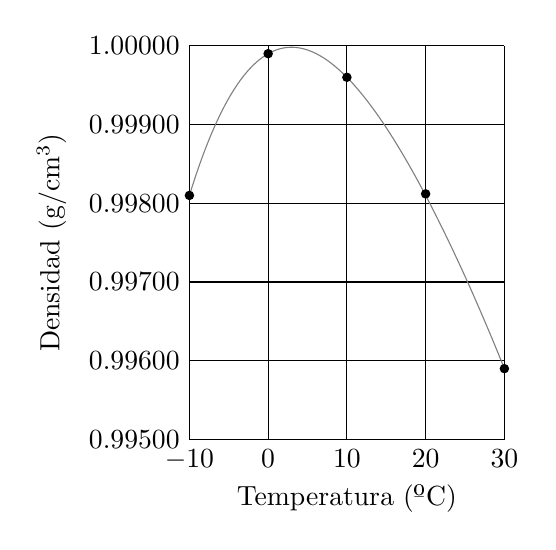
\begin{tikzpicture}
            \draw (0,0) grid (4,5);
            \foreach \i in {-1,1,2,3}
            \node[below] at (\i+1,0) {$\i 0$};
            \node[below] at (1,0) {$0$};
            \foreach \j in {5,6,7,8,9}
            \node[left] at (0,\j-5) {$0.99 \j 00$};
            \node[left] at (0,5) {$1.00000$};
            \draw[gray, domain=0:4, samples=100] plot(\x,{-0.0166666666667*\x^4 + 0.25*\x^3 - 1.683333333333*\x^2 + 3.25*\x + 3.1});
            \filldraw (0,3.1) circle (1.5pt);
            \filldraw (1,4.9) circle (1.5pt);
            \filldraw (2,4.6) circle (1.5pt);
            \filldraw (3,3.12) circle (1.5pt);
            \filldraw (4,0.9) circle (1.5pt);
            \node at (2,-0.75) {Temperatura (º$\mathrm{C}$)};
            \node[rotate=90] at (-1.75,2.5) {Densidad ($\mathrm{g}/\mathrm{cm}^3$)};
        \end{tikzpicture}
    \end{center}\newpage\noindent
    En dicha figura, vemos que el máximo se alcanza en el intervalo $[0, 10]$. Para encontrar este máximo, igualamos $S'(x)$ a cero en el intervalo $[0, 10]$:
    $$S'(x) = 0.000000339x^2 - 0.0001974x + 0.0000733 = 0$$
    Con tres cifras significativas, la raíz de esta ecuación cuadrática en el intervalo $[0, 10]$ es $x = 3.99$, y para este valor de $x$, $S(3.99) = 1.00001$. Así, según nuestra estimación interpolada, la densidad máxima del agua es $1.00001$ $\mathrm{g}/\mathrm{cm}^3$ alcanzada a $3.99$º$\mathrm{C}$. Esto concuerda bien con la densidad máxima experimental de $1.00000$ $\mathrm{g}/\mathrm{cm}^3$ alcanzada a $3.98$º$\mathrm{C}$.
\end{example}

En conclusión, además de producir excelentes curvas de interpolación, los splines cúbicos y sus generalizaciones son útiles para la integración y diferenciación numérica, para la solución numérica de ecuaciones diferenciales e integrales, y en la teoría de la optimización.

\section{Cadenas de Markov}

Supongamos que un sistema físico o matemático atraviesa un proceso de cambio de tal manera que en cualquier momento puede ocupar uno de un número finito de estados. Por ejemplo, el clima en una ciudad determinada podría estar en uno de tres posibles estados: soleado, nublado o lluvioso. O imaginemos que un individuo podría estar en uno de cuatro posibles estados emocionales: feliz, triste, enojado o aprensivo. Supongamos que tal sistema cambia con el tiempo de un estado a otro y que en momentos programados se observa el estado del sistema. Si el estado del sistema en una observación no puede predecirse con certeza, pero la probabilidad de que ocurra un estado dado puede predecirse simplemente conociendo el estado del sistema en la observación precedente, entonces el proceso de cambio se llama \emph{cadena de Markov} o \emph{proceso de Markov}.

\begin{definition}
    Si una cadena de Markov tiene $k$ posibles estados, etiquetados como $1, 2, \ldots, k$, entonces la probabilidad de que el sistema esté en el estado $i$ en una observación, después de haber estado en el estado $j$ en la observación anterior, se denota por $p_{ij}$ y se llama probabilidad de transición del estado $j$ al estado $i$. La matriz $P = \llparenthesis p_{ij} \rrparenthesis$ se llama \emph{matriz de transición de la cadena de Markov}.
\end{definition}

Por ejemplo, en una cadena de Markov de tres estados, la matriz de transición tiene la forma\\
\begin{nscenter}
    \begin{tikzpicture}
        \node (A) at (0,0) {$\begin{bmatrix} p_{11} & p_{12} & p_{13} \\ p_{21} & p_{22} & p_{23} \\ p_{31} & p_{32} & p_{33} \end{bmatrix}$};
        \node[black!90!white, xshift=-0.85cm, yshift=0.1cm] at (A.north) {$1$};
        \node[black!90!white, yshift=0.1cm] at (A.north) {$2$};
        \node[black!90!white, xshift=0.85cm, yshift=0.1cm] at (A.north) {$3$};
        \node[black!90!white,yshift=0.4cm] at (A.east) {$1$};
        \node[black!90!white] at (A.east) {$2$};
        \node[black!90!white,yshift=-0.4cm] at (A.east) {$3$};
        \node[yshift=0.75cm] at (A.north) {Estado precedente};
        \node[right,xshift=0.5cm] at (A.east) {Nuevo estado};
    \end{tikzpicture}
\end{nscenter}
En esta matriz, $p_{32}$ es la probabilidad de que el sistema cambie del estado $2$ al estado $3$, $p_{11}$ es la probabilidad de que el sistema permanezca en el estado $1$ si estaba previamente en el estado $1$, y así sucesivamente.

\begin{example}\label{exam:markov1}
    Una agencia de alquiler de coches tiene tres ubicaciones de alquiler, denominadas $1$, $2$ y $3$. Un cliente puede alquilar un coche en cualquiera de las tres ubicaciones y devolverlo a cualquiera de las tres ubicaciones. El gerente encuentra que los clientes devuelven los coches a las diversas ubicaciones según las siguientes probabilidades:\newpage
    \begin{nscenter}
        \begin{tikzpicture}
            \node (A) at (0,0) {$\begin{bmatrix} 0.8 & 0.3 & 0.2 \\ 0.1 & 0.2 & 0.6 \\ 0.1 & 0.5 & 0.2 \end{bmatrix}$};
            \node[black!90!white, xshift=-0.85cm, yshift=0.1cm] at (A.north) {$1$};
            \node[black!90!white, yshift=0.1cm] at (A.north) {$2$};
            \node[black!90!white, xshift=0.85cm, yshift=0.1cm] at (A.north) {$3$};
            \node[black!90!white,yshift=0.4cm] at (A.east) {$1$};
            \node[black!90!white] at (A.east) {$2$};
            \node[black!90!white, yshift=-0.4cm] at (A.east) {$3$};
            \node[yshift=0.75cm] at (A.north) {Alquilado desde la ubicación};
            \node[right,xshift=0.5cm] at (A.east) {\makecell{Regresado \\ a la \\ ubicación}};
        \end{tikzpicture}
    \end{nscenter}
    Esta matriz es la matriz de transición del sistema considerado como una cadena de Markov. De esta matriz, se puede ver que la probabilidad de que un coche alquilado en la ubicación $3$ sea devuelto a la ubicación $2$ es de $0.3$, la probabilidad de que un coche alquilado en la ubicación $1$ sea devuelto a la ubicación $1$ es de $0.5$, y así sucesivamente.
\end{example}

\begin{example}\label{exam:markov2}
    Al revisar los registros de donaciones, la oficina de exalumnos de una universidad descubre que el $80\%$ de sus exalumnos que contribuyen al fondo anual un año también contribuirán al siguiente año, y el $30\%$ de aquellos que no contribuyen un año contribuirán al siguiente. Esto se puede ver como una cadena de Markov con dos estados: el estado $1$ corresponde a un exalumno que dona en un año determinado, y el estado $2$ corresponde a un exalumno que no dona en ese año. La matriz de transición es
    $$P = \begin{bmatrix}
        0.80 & 0.30 \\
        0.20 & 0.70
    \end{bmatrix}$$
\end{example}

En los ejemplos anteriores, las matrices de transición de las cadenas de Markov tienen la propiedad de que la suma de las entradas en cualquier columna es igual a $1$. Esto no es accidental. Si $P = \llparenthesis p_{ij} \rrparenthesis$ es la matriz de transición de cualquier cadena de Markov con $k$ estados, entonces para cada $j$ debemos tener
\begin{equation}
    p_{1j} + p_{2j} + \cdots + p_{kj} = 1 \label{IAUAUAIQIOQPQOQJQCCCAHAIAIAIA}
\end{equation}
porque si el sistema está en el estado $j$ en una observación, es seguro que estará en uno de los $k$ estados posibles en la siguiente observación.

Una matriz con la propiedad \eqref{IAUAUAIQIOQPQOQJQCCCAHAIAIAIA} se llama \emph{matriz estocástica}, \emph{matriz de probabilidad} o \emph{matriz de Markov}. De la discusión anterior, se sigue que la matriz de transición para una cadena de Markov debe ser una matriz estocástica.

En una cadena de Markov, el estado del sistema en cualquier momento de observación generalmente no puede determinarse con certeza. Lo mejor que se puede hacer normalmente es especificar probabilidades para cada uno de los estados posibles. Por ejemplo, en una cadena de Markov con tres estados, podríamos describir el estado posible del sistema en algún momento de observación mediante un vector columna
$$
\mathbb{x} = \begin{bmatrix}
    x_1 \\
    x_2 \\
    x_3
\end{bmatrix}
$$
en el que $x_1$ es la probabilidad de que el sistema esté en el estado $1$, $x_2$ es la probabilidad de que esté en el estado $2$, y $x_3$ es la probabilidad de que esté en el estado $3$. En general, tenemos la siguiente definición.

\begin{definition}
    El \emph{vector de estado} para una observación de una cadena de Markov con $k$ estados es un vector columna $\mathbb{x}$, cuya $i$-ésima componente $x_i$ es la probabilidad de que el sistema esté en el estado $i$ en ese momento.
\end{definition}

Observe que las entradas en cualquier vector de estado para una cadena de Markov son no negativas y suman $1$ (¿por qué?). Un vector columna que tiene esta propiedad se llama \emph{vector de probabilidad}. Supongamos ahora que conocemos el vector de estado $\mathbb{x}^{(0)}$ para una cadena de Markov en alguna observación inicial. El siguiente teorema nos permitirá determinar los vectores de estado
$$\mathbb{x}^{(1)}, \mathbb{x}^{(2)}, \dots, \mathbb{x}^{(n)}, \dots$$
en los tiempos de observación subsiguientes.

\begin{theorem}\label{theo:matrix_transition-state}
    Si $P$ es la matriz de transición de una cadena de Markov y $\mathbb{x}^{(n)}$ es el vector de estado en la $n$-ésima observación, entonces $\mathbb{x}^{(n+1)} = P \mathbb{x}^{(n)}$.
\end{theorem}

La demostración del anterior teorema involucra ideas de teoría de probabilidad y no será presentada aquí. A partir de este teorema, se sigue que
\begin{align*}
    \mathbb{x}^{(1)} & = P\mathbb{x}^{(0)} \\
    \mathbb{x}^{(2)} & = P\mathbb{x}^{(1)} = P^2\mathbb{x}^{(0)} \\
    \mathbb{x}^{(3)} & = P\mathbb{x}^{(2)} = P^3\mathbb{x}^{(0)} \\
    & \vdots \\
    \mathbb{x}^{(n)} & = P\mathbb{x}^{(n-1)} = P^n\mathbb{x}^{(0)}
\end{align*}
De esta manera, el vector de estado inicial $\mathbb{x}^{(0)}$ y la matriz de transición $P$ determinan $\mathbb{x}^{(n)}$ para $n = 1, 2, \dots$.

\begin{example}\label{exam:markov3}
    La matriz de transición en el ejemplo \ref{exam:markov2} era
    $$P = \begin{bmatrix}
        0.8 & 0.3 \\
        0.2 & 0.7
    \end{bmatrix}$$
    Ahora construimos el probable registro futuro de donaciones de un nuevo graduado que no hizo una donación en el año inicial después de la graduación. Para tal graduado, el sistema está inicialmente en el estado $2$ con certeza, por lo que el vector de estado inicial es
    $$\mathbb{x}^{(0)} = \begin{bmatrix} 0 \\ 1 \end{bmatrix}$$
    A partir del teorema \ref{theo:matrix_transition-state}, tenemos entonces
    \begin{align*}
        \mathbb{x}^{(1)} & = P\mathbb{x}^{(0)} = \begin{bmatrix} 0.8 & 0.3 \\ 0.2 & 0.7 \end{bmatrix} \begin{bmatrix} 0 \\ 1 \end{bmatrix} = \begin{bmatrix} 0.3 \\ 0.7 \end{bmatrix} \\
        \mathbb{x}^{(2)} & = P\mathbb{x}^{(1)} = \begin{bmatrix} 0.8 & 0.3 \\ 0.2 & 0.7 \end{bmatrix} \begin{bmatrix} 0.3 \\ 0.7 \end{bmatrix} = \begin{bmatrix} 0.45 \\ 0.55 \end{bmatrix} \\
        \mathbb{x}^{(3)} & = P\mathbb{x}^{(2)} = \begin{bmatrix} 0.8 & 0.3 \\ 0.2 & 0.7 \end{bmatrix} \begin{bmatrix} 0.45 \\ 0.55 \end{bmatrix} = \begin{bmatrix} 0.525 \\ 0.475 \end{bmatrix}
    \end{align*}
    Así, después de tres años, se espera que el exalumno haga una donación con una probabilidad de $0.525$. Más allá de tres años, encontramos los siguientes vectores de estado (con tres decimales):
    \begin{align*}
        \mathbb{x}^{(4)} & = \begin{bmatrix} 0.563 \\ 0.438 \end{bmatrix}, & \mathbb{x}^{(5)} & = \begin{bmatrix} 0.581 \\ 0.419 \end{bmatrix}, & \mathbb{x}^{(6)} & = \begin{bmatrix} 0.591 \\ 0.409 \end{bmatrix}, & \mathbb{x}^{(7)} & = \begin{bmatrix} 0.595 \\ 0.405 \end{bmatrix}, \\
        \mathbb{x}^{(8)} & = \begin{bmatrix} 0.598 \\ 0.402 \end{bmatrix}, & \mathbb{x}^{(9)} & = \begin{bmatrix} 0.599 \\ 0.401 \end{bmatrix}, & \mathbb{x}^{(10)} & = \begin{bmatrix} 0.599 \\ 0.401 \end{bmatrix}, & \mathbb{x}^{(11)} & = \begin{bmatrix} 0.600 \\ 0.400 \end{bmatrix}
    \end{align*}
    Para todos los $n$ mayores de $11$, tenemos
    $$\mathbb{x}^{(n)} = \begin{bmatrix} 0.600 \\ 0.400 \end{bmatrix}$$
    con tres decimales. En otras palabras, los vectores de estado convergen a un vector fijo a medida que aumenta el número de observaciones.
\end{example}

\newpage

\begin{example}
    La matriz de transición en el ejemplo \ref{exam:markov1} era
    $$\begin{bmatrix}
        0.8 & 0.3 & 0.2 \\
        0.1 & 0.2 & 0.6 \\
        0.1 & 0.5 & 0.2
    \end{bmatrix}$$
    Si un auto se alquila inicialmente desde la ubicación $2$, entonces el vector de estado inicial es
    $$\mathbb{x}^{(0)} = \begin{bmatrix}
        0 \\
        1 \\
        0
    \end{bmatrix}$$
    Usando este vector y el teorema \ref{theo:matrix_transition-state}, se obtienen los siguientes vectores de estado que se enumeran en la siguiente tabla:
    \begin{table*}[h!]
        \centering
        \begin{NiceTabular}{ccccccccccccc}[vlines,cell-space-limits=4pt]
            \CodeBefore
            \rowcolor{black!20!white}{1}
            \columncolor{black!20!white}{1}
            \rowcolor{black!20!white}{2}
            \Body
            \hline
            \Block{2-1}{\diagbox{\raisebox{4pt}{\hspace*{0.1cm} $\mathbb{x}^{(n)}$}}{\raisebox{-0.4cm}{$n$\hspace{0.3cm}}}} & \Block{2-1}{$0$} & \Block{2-1}{$1$} & \Block{2-1}{$2$} & \Block{2-1}{$3$} & \Block{2-1}{$4$} & \Block{2-1}{$5$} & \Block{2-1}{$6$} & \Block{2-1}{$7$} & \Block{2-1}{$8$} & \Block{2-1}{$9$} & \Block{2-1}{$10$} & \Block{2-1}{$11$}\\
            \hspace{1.5cm} & \\
            \hline
            $x_1^{(n)}$ & $0$ & $0.300$ & $0.400$ & $0.477$ & $0.511$ & $0.533$ & $0.544$ & $0.550$ & $0.553$ & $0.555$ & $0.556$ & $0.557$ \\
            $x_2^{(n)}$ & $1$ & $0.200$ & $0.370$ & $0.252$ & $0.261$ & $0.240$ & $0.238$ & $0.233$ & $0.232$ & $0.231$ & $0.230$ & $0.230$ \\
            $x_3^{(n)}$ & $0$ & $0.500$ & $0.230$ & $0.271$ & $0.228$ & $0.227$ & $0.219$ & $0.217$ & $0.215$ & $0.214$ & $0.214$ & $0.213$ \\
            \hline
        \end{NiceTabular}
        \caption{~}
        \label{table:markov1}
    \end{table*}\vspace{-0.5cm}
    
    Para todos los valores de $n$ mayores a $11$, todos los vectores de estado son iguales a $\mathbb{x}^{(11)}$ con tres decimales.
    
    Se deben observar dos cosas en este ejemplo. Primero, no era necesario saber cuánto tiempo un cliente mantenía el coche. Es decir, en un proceso de Markov, el período de tiempo entre observaciones no necesita ser regular. Segundo, los vectores de estado se aproximan a un vector fijo a medida que $n$ aumenta.
\end{example}

\begin{example}\label{exam:markov5}
    \sideFigure[\label{fig:police}]{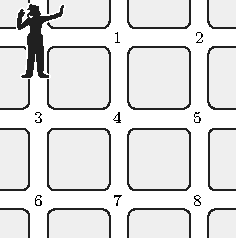
\includegraphics[width=\linewidth]{Images/Capitulo8/Police.pdf}}Una oficial de tráfico está asignada a controlar el tráfico en las ocho intersecciones indicadas en la figura \ref{fig:police}. Se le instruye permanecer en cada intersección durante una hora y luego, ya sea permanecer en la misma intersección o moverse a una intersección vecina. Para evitar establecer un patrón, se le indica elegir su nueva intersección de manera aleatoria, con cada elección posible igualmente probable. Por ejemplo, si se encuentra en la intersección $5$, su próxima intersección puede ser $2$, $4$, $5$, o $8$, cada una con una probabilidad de $1/4$. Cada día, comienza en el lugar donde se detuvo el día anterior. La matriz de transición para esta cadena de Markov es:\\
    \begin{nscenter}
        \begin{tikzpicture}
            \node (A) at (0,0) {$\begin{bmatrix} 1/3 & 1/3 & 0 & 1/5 & 0 & 0 & 0 & 0 \\ 1/3 & 1/3 & 0 & 0 & 1/4 & 0 & 0 & 0 \\ 0 & 0 & 1/3 & 1/5 & 0 & 1/3 & 0 & 0 \\ 1/3 & 0 & 1/3 & 1/5 & 1/4 & 0 & 1/4 & 0 \\ 0 & 1/3 & 0 & 1/5 & 1/4 & 0 & 0 & 1/3 \\ 0 & 0 & 1/3 & 0 & 0 & 1/3 & 1/4 & 0 \\ 0 & 0 & 0 & 1/5 & 0 & 1/3 & 1/4 & 1/3 \\ 0 & 0 & 0 & 0 & 1/4 & 0 & 1/4 & 1/3 \end{bmatrix}$};
            \foreach \i in {1,2,3,...,8}
            {
            \node[black!90!white, xshift=-3.95cm+\i*0.88cm, yshift=0.1cm] at (A.north) {$\i$};
            \node[black!90!white, yshift=1.9cm-\i*0.416cm] at (A.east) {$\i$};
            }
            \node[yshift=0.75cm] at (A.north) {Antigua intersección};
            \node[right,xshift=0.5cm] at (A.east) {Nueva intersección};
        \end{tikzpicture}
    \end{nscenter}
    Si la oficial de tráfico comienza en la intersección $5$, sus ubicaciones probables, hora por hora, están dadas por los vectores de estado que se muestran en la tabla \ref{table:markov2}. Para todos los valores de $n$ mayores que $22$, todos los vectores de estado son iguales a $\mathbb{x}^{(22)}$ con tres decimales. Así, al igual que en los dos primeros ejemplos, los vectores de estado se acercan a un vector fijo a medida que $n$ aumenta.\newpage
    \begin{table*}[h!]
        \centering
        \begin{NiceTabular}{cccccccccccccc}[vlines,cell-space-limits=4pt]
            \CodeBefore
            \rowcolor{black!20!white}{1}
            \columncolor{black!20!white}{1}
            \rowcolor{black!20!white}{2}
            \Body
            \hline
            \Block{2-1}{\diagbox{\raisebox{4pt}{\hspace*{0.1cm} $\mathbb{x}^{(n)}$}}{\raisebox{-0.4cm}{$n$\hspace{0.3cm}}}} & \Block{2-1}{$0$} & \Block{2-1}{$1$} & \Block{2-1}{$2$} & \Block{2-1}{$3$} & \Block{2-1}{$4$} & \Block{2-1}{$5$} & \Block{2-1}{$\cdots$} & \Block{2-1}{$10$} & \Block{2-1}{$\cdots$} & \Block{2-1}{$15$} & \Block{2-1}{$\cdots$} & \Block{2-1}{$21$} & \Block{2-1}{$22$} \\
            \hspace{1.5cm} & \\
            \hline
            $x_1^{(n)}$ & $0$ & $0.000$ & $0.133$ & $0.116$ & $0.130$ & $0.123$ & $\cdots$ & $0.113$ & $\cdots$ & $0.109$ & $\cdots$ & $0.108$ & $0.107$ \\
            $x_2^{(n)}$ & $0$ & $0.250$ & $0.146$ & $0.163$ & $0.140$ & $0.138$ & $\cdots$ & $0.115$ & $\cdots$ & $0.109$ & $\cdots$ & $0.108$ & $0.107$ \\
            $x_3^{(n)}$ & $0$ & $0.000$ & $0.050$ & $0.039$ & $0.067$ & $0.073$ & $\cdots$ & $0.100$ & $\cdots$ & $0.106$ & $\cdots$ & $0.107$ & $0.107$ \\
            $x_4^{(n)}$ & $0$ & $0.250$ & $0.113$ & $0.187$ & $0.162$ & $0.178$ & $\cdots$ & $0.178$ & $\cdots$ & $0.179$ & $\cdots$ & $0.179$ & $0.179$ \\
            $x_5^{(n)}$ & $1$ & $0.250$ & $0.279$ & $0.190$ & $0.190$ & $0.168$ & $\cdots$ & $0.149$ & $\cdots$ & $0.144$ & $\cdots$ & $0.143$ & $0.143$ \\
            $x_6^{(n)}$ & $0$ & $0.000$ & $0.000$ & $0.050$ & $0.056$ & $0.074$ & $\cdots$ & $0.099$ & $\cdots$ & $0.105$ & $\cdots$ & $0.107$ & $0.107$ \\
            $x_7^{(n)}$ & $0$ & $0.000$ & $0.133$ & $0.104$ & $0.131$ & $0.125$ & $\cdots$ & $0.138$ & $\cdots$ & $0.142$ & $\cdots$ & $0.143$ & $0.143$ \\
            $x_8^{(n)}$ & $0$ & $0.250$ & $0.146$ & $0.152$ & $0.124$ & $0.121$ & $\cdots$ & $0.108$ & $\cdots$ & $0.107$ & $\cdots$ & $0.107$ & $0.107$ \\
            \hline
        \end{NiceTabular}
        \caption{~}
        \label{table:markov2}
    \end{table*}\vspace{-0.5cm}
\end{example}

En nuestros ejemplos vimos que los vectores de estado se aproximaban a un vector fijo a medida que aumentaba el número de observaciones. Ahora nos preguntamos si los vectores de estado siempre se aproximan a un vector fijo en una cadena de Markov. Un ejemplo sencillo muestra que este no es siempre el caso.

\begin{example}
    Sean
    $$P = \begin{bmatrix}
        0 & 1 \\
        1 & 0
    \end{bmatrix} \quad \text{ y } \quad \mathbb{x}^{(0)} = \begin{bmatrix}
        1 \\
        0
    \end{bmatrix}$$
    Entonces, dado que $P^2 = I_2$ y $P^3 = P$, tenemos que
    $$\mathbb{x}^{(0)} = \mathbb{x}^{(2)} = \mathbb{x}^{(4)} = \cdots = \begin{bmatrix} 1 \\ 0 \end{bmatrix}$$
    y
    $$\mathbb{x}^{(1)} = \mathbb{x}^{(3)} = \mathbb{x}^{(5)} = \cdots = \begin{bmatrix} 0 \\ 1 \end{bmatrix}$$
    Este sistema oscila indefinidamente entre los dos vectores $\begin{bmatrix} 0 \\ 1 \end{bmatrix}$ y $\begin{bmatrix} 1 \\ 0 \end{bmatrix}$, por lo que no se aproxima a ningún vector fijo.
\end{example}

No obstante, si imponemos una condición simple a la matriz de transición, podemos demostrar que se alcanza un vector de estado fijo. Esta condición se define a continuación.

\begin{definition}
    Una matriz de transición se considera \emph{regular} si, al elevarla a alguna potencia entera, todas sus entradas son positivas.
\end{definition}

Por lo tanto, para una matriz de transición regular $P$, existe un entero positivo $m$ tal que todas las entradas de $P^m$ son positivas. Este es el caso de las matrices de transición en los ejemplos \ref{exam:markov1} y \ref{exam:markov2} con $m = 1$. En el ejemplo \ref{exam:markov5}, resulta que $P^4$ tiene todas las entradas positivas. Por lo tanto, en los tres ejemplos, las matrices de transición son regulares.

Una cadena de Markov con una matriz de transición regular se llama \emph{cadena de Markov regular}. Veremos que toda cadena de Markov regular tiene un vector de estado fijo $\mathbb{q}$ tal que $P^n \mathbb{x}^{(0)}$ se aproxima a $\mathbb{q}$ a medida que $n$ aumenta, para cualquier elección de $\mathbb{x}^{(0)}$. Este resultado es de gran importancia en la teoría de cadenas de Markov y se basa en el siguiente teorema.

\newpage
\infoBulle{No demostraremos este teorema aquí. Para una demostración detallada, consulte un texto más especializado, como J. Kemeny y J. Snell, \emph{Finite Markov Chains} (New York: Springer-Verlag, 1976).}

\begin{theorem}\label{theo:tomarkov2}
    Si $P$ es una matriz de transición regular, entonces a medida que $n \to \infty$,
    $$P^n \to \begin{bmatrix}
        q_1 & q_1 & \cdots & q_1 \\
        q_2 & q_2 & \cdots & q_2 \\
        \vdots & & \ddots & \vdots \\
        q_k & q_k & \cdots & q_k
    \end{bmatrix}$$
    donde los $q_i$ son números positivos tales que $q_1 + q_2 + \cdots + q_k = 1$.
\end{theorem}

Consideremos
$$Q = \begin{bmatrix}
    q_1 & q_1 & \cdots & q_1 \\
    q_2 & q_2 & \cdots & q_2 \\
    \vdots & & \ddots & \vdots \\
    q_k & q_k & \cdots & q_k
\end{bmatrix} \quad \text{ y } \quad \mathbb{q} = \begin{bmatrix}
    q_1 \\
    q_2 \\
    \vdots \\
    q_k
\end{bmatrix}$$
Es decir, $Q$ es una matriz de transición cuyas columnas son todas iguales al vector de probabilidad $\mathbb{q}$. $Q$ tiene la propiedad de que si $\mathbb{x}$ es cualquier vector de probabilidad, entonces
\begin{align*}
    Q\mathbb{x} & = \begin{bmatrix}
        q_1 & q_1 & \cdots & q_1 \\
        q_2 & q_2 & \cdots & q_2 \\
        \vdots & & \ddots & \vdots \\
        q_k & q_k & \cdots & q_k
    \end{bmatrix} \begin{bmatrix}
        x_1 \\
        x_2 \\
        \vdots \\
        x_k
    \end{bmatrix} \\
    & = \begin{bmatrix}
        q_1x_1 + q_1x_2 + \cdots + q_1x_k \\
        q_2x_1 + q_2x_2 + \cdots + q_2x_k \\
        \vdots \\
        q_kx_1 + q_kx_2 + \cdots + q_kx_k
    \end{bmatrix} \\
    & = (x_1 + x_2 + \cdots + x_k) \begin{bmatrix}
        q_1 \\
        q_2 \\
        \vdots \\
        q_k
    \end{bmatrix} \\
    & = (1) \mathbb{q} \\
    & = \mathbb{q}
\end{align*}
Es decir, $Q$ transforma cualquier vector de probabilidad $\mathbb{x}$ en el vector de probabilidad fijo $\mathbb{q}$. Este resultado nos lleva al siguiente teorema.

\begin{theorem}\label{theo:tomarkov3}
    Si $P$ es una matriz de transición regular y $\mathbb{x}$ es cualquier vector de probabilidad, entonces, conforme $n \to \infty$, 
    $$P^n \mathbb{x} \to \begin{bmatrix}
        q_1 \\
        q_2 \\
        \vdots \\
        q_k
    \end{bmatrix} = \mathbb{q}$$
    donde $\mathbb{q}$ es un vector de probabilidad fijo, independiente de $n$, y cuyos componentes son todos positivos.
\end{theorem}

Este resultado se cumple ya que el teorema \ref{theo:tomarkov2} implica que $P^n \to Q$ a medida que $n \to \infty$. Esto, a su vez, implica que $P^n\mathbb{x} \to Q\mathbb{x} = \mathbb{q}$ a medida que $n \to \infty$. Así, para una cadena de Markov regular, el sistema eventualmente se aproxima a un vector de estado fijo $\mathbb{q}$. Este vector $\mathbb{q}$ se llama el \emph{vector de estado estacionario} de la cadena de Markov regular.

Para sistemas con muchos estados, usualmente la técnica más eficiente para calcular el vector de estado estacionario $\mathbb{q}$ es simplemente calcular $P^n \mathbb{x}$ para algún $n$ grande. Nuestros ejemplos ilustran este procedimiento. Cada uno es un proceso de Markov regular, por lo que la convergencia a un vector de estado estacionario está asegurada. Otra forma de calcular el vector de estado estacionario es utilizando el siguiente teorema.

\begin{theorem}\label{theo:tomarkov4}
    El vector de estado estacionario $\mathbb{q}$ de una matriz de transición regular $P$ es el único vector de probabilidad que satisface la ecuación $P \mathbb{q} = \mathbb{q}$.
\end{theorem}

Para entender esto, consideremos la identidad matricial $PP^n = P^{n+1}$. Según el teorema \ref{theo:tomarkov2}, tanto $P^n$ como $P^{n+1}$ se aproximan a $Q$ a medida que $n \to \infty$. Así, tenemos $PQ = Q$. Cualquier columna de esta ecuación matricial da como resultado $P\mathbb{q} = \mathbb{q}$. Para demostrar que $\mathbb{q}$ es el único vector de probabilidad que satisface esta ecuación, supongamos que $\mathbb{r}$ es otro vector de probabilidad tal que $P\mathbb{r} = \mathbb{r}$. Entonces también $P^n\mathbb{r} = \mathbb{r}$ para $n = 1, 2, \dots$. Cuando dejamos que $n \to \infty$, el teorema \ref{theo:tomarkov3} nos lleva a que $\mathbb{q} = \mathbb{r}$.

La ecuación del teorema \ref{theo:tomarkov4} también se puede expresar como un sistema lineal homogéneo
$$(I_k - P)\mathbb{q} = \mathbb{0}$$
donde tiene una solución única, el vector $\mathbb{q}$, con entradas no negativas que satisfacen la condición $q_1 + q_2 + \cdots + q_k = 1$. Podemos aplicar esta técnica para calcular los vectores de estado estacionario en nuestros ejemplos.

\begin{example}
    En el ejemplo \ref{exam:markov2}, la matriz de transición era
    $$P = \begin{bmatrix} 
        0.8 & 0.3 \\ 
        0.2 & 0.7 
    \end{bmatrix}$$
    Entonces, el sistema lineal $(I_2 - P)\mathbb{q} = \mathbb{0}$ es
    $$\begin{bmatrix*}[r]
        0.2 & -0.3 \\
        -0.2 & 0.3
    \end{bmatrix*}\begin{bmatrix}
        q_1 \\
        q_2
    \end{bmatrix} = \begin{bmatrix}
        0 \\
        0
    \end{bmatrix}$$
    Esto lleva a la única ecuación independiente
    $$0.2q_1 - 0.3q_2 = 0$$
    o bien,
    $$q_1 = 1.5q_2$$
    Es decir, la solución general al sistema está dada por
    $$\mathbb{q} = \begin{bmatrix}
        1.5q_2 \\
        q_2
    \end{bmatrix} = q_2 \begin{bmatrix}
        1.5 \\
        1
    \end{bmatrix}$$
    Para que el vector $\mathbb{q}$ sea un vector de probabilidad, la suma de las entradas de $\mathbb{q}$ debe ser igual a $1$. Así,
    $$q_2 = \frac{1}{1.5 + 1} = 0.4$$
    Por consiguiente,
    $$\mathbb{q} = \begin{bmatrix}
        0.6 \\
        0.4
    \end{bmatrix}$$
    es el vector de estado estacionario de esta cadena de Markov regular. Esto significa que a largo plazo, el $60\%$ de los exalumnos harán una donación en un año determinado, y el $40\%$ no lo harán. Observe que esto concuerda con el resultado obtenido numéricamente en el ejemplo \ref{exam:markov3}.
\end{example}

\newpage

\begin{example}
    En el ejemplo \ref{exam:markov1}, la matriz de transición era
    $$P = \begin{bmatrix}
        0.8 & 0.3 & 0.2 \\
        0.1 & 0.2 & 0.6 \\
        0.1 & 0.5 & 0.2
    \end{bmatrix}$$
    Así que el sistema lineal $(I_3 - P)\mathbb{q} = \mathbb{0}$ está dado por
    $$\begin{bmatrix*}[r]
        0.2 & -0.3 & -0.2 \\
        -0.1 & 0.8 & -0.6 \\
        -0.1 & -0.5 & 0.8
    \end{bmatrix*}\begin{bmatrix}
        q_1 \\
        q_2 \\
        q_3
    \end{bmatrix} = \begin{bmatrix}
        0 \\
        0 \\
        0
    \end{bmatrix}$$
    Utilizando el método de reducción de Gauss-Jordan, obtenemos que
    $$\begin{bmatrix}
        1 & 0 & -\dfrac{34}{13} \\[3mm]
        0 & 1 & -\dfrac{14}{13} \\[3mm]
        0 & 0 & \phantom{-}0
    \end{bmatrix}\begin{bmatrix}
        q_1 \\
        q_2 \\
        q_3
    \end{bmatrix} = \begin{bmatrix}
        0 \\
        0 \\
        0
    \end{bmatrix}$$
    Por lo que el sistema lineal original es equivalente al sistema
    \begin{align*}
        q_1 & = \frac{34}{13} q_3 \\
        q_2 & = \frac{14}{13} q_3
    \end{align*}
    Es decir, la solución general al sistema está dada por
    $$\mathbb{q} = \begin{bmatrix}
        \dfrac{34}{13} q_3 \\[3mm]
        \dfrac{14}{13} q_3 \\[3mm]
        q_3
    \end{bmatrix} = q_3 \begin{bmatrix}
        \dfrac{34}{13} \\[3mm] 
        \dfrac{14}{13} \\[3mm]
        1
    \end{bmatrix}$$
    Para que el vector $\mathbb{q}$ sea un vector de probabilidad, la suma de las entradas de $\mathbb{q}$ debe ser igual a $1$. Así,
    $$q_3 = \frac{1}{\dfrac{34}{13} + \dfrac{14}{13} + 1} = \frac{13}{61}$$
    Por consiguiente, el vector de estado estacionario del sistema es
    $$\mathbb{q} = \begin{bmatrix}
        \dfrac{34}{61} \\[2mm]
        \dfrac{14}{61} \\[2mm]
        \dfrac{13}{61}
    \end{bmatrix} = \begin{bmatrix}
        0.5573 \dots \\
        0.2295 \dots \\
        0.2131 \dots
    \end{bmatrix}$$
    Esto concuerda con el resultado obtenido numéricamente en la tabla \ref{table:markov1}. Los valores de $\mathbb{q}$ dan las probabilidades a largo plazo de que cualquier coche sea devuelto a la ubicación $1$, $2$ o $3$, respectivamente. Si la agencia de alquiler de coches tiene una flota de $1 \, 000$ coches, debería diseñar sus instalaciones de manera que haya al menos $558$ espacios en la ubicación $1$, al menos $230$ espacios en la ubicación $2$, y al menos $214$ espacios en la ubicación $3$.
\end{example}

\begin{example}
    Tomemos la matriz de transición del ejemplo \ref{exam:markov5}. No daremos los detalles de los cálculos, pero simplemente afirmaremos que la única solución del vector de probabilidad para el sistema lineal $(I_8 - P)\mathbb{q} = \mathbb{0}$ es\newpage
    $$\mathbb{q} = \frac{1}{28} \begin{bmatrix}
        3 \\
        3 \\
        3 \\
        5 \\
        4 \\
        3 \\
        4 \\
        3
    \end{bmatrix} = \begin{bmatrix}
        0.1071\dots \\
        0.1071\dots \\
        0.1071\dots \\
        0.1785\dots \\
        0.1428\dots \\
        0.1071\dots \\
        0.1428\dots \\
        0.1071\dots \\
    \end{bmatrix}$$
    Esto concuerda con el resultado obtenido numéricamente en la tabla \ref{table:markov2}. Los valores de este vector muestran la proporción de tiempo que la oficial de tráfico pasa en cada intersección a largo plazo. Por lo tanto, si se busca que pase la misma cantidad de tiempo en todas las intersecciones, la estrategia de moverse aleatoriamente con probabilidades iguales entre intersecciones no es adecuada.
\end{example}

\section{Teoría de grafos}

Existen innumerables ejemplos de conjuntos finitos donde sus elementos están relacionados de alguna manera. Por ejemplo, el conjunto podría estar compuesto por personas, animales, países, empresas, equipos deportivos o ciudades. La relación entre dos elementos, $A$ y $B$, podría ser que la persona $A$ domina a la persona $B$, el animal $A$ se alimenta del animal $B$, el país $A$ apoya militarmente al país $B$, la empresa $A$ vende su producto a la empresa $B$, el equipo deportivo $A$ siempre vence al equipo deportivo $B$, o la ciudad $A$ tiene un vuelo directo a la ciudad $B$.

Ahora mostraremos cómo la teoría de \emph{grafos dirigidos} puede utilizarse para modelar matemáticamente relaciones como estas.

\subsection*{Grafos dirigidos}
\sideFigure[\label{fig:examgrafos1}]{
\begin{tikzpicture}
    %%%%% COORDENADAS %%%%%
    \coordinate (P1) {};
    \coordinate[above right=1cm and 2.5cm of P1] (P2) {};
    \coordinate[below right=1.1cm and 0.5cm of P2] (P3) {};
    \coordinate[below left=1.25cm and 0.1cm of P3] (P4) {};
    \coordinate[above left=0.25cm and 1.75cm of P4] (P5) {};
    \coordinate[above right=0.5cm and 3cm of P5] (P6) {};
    \coordinate[above left=1.25cm and 0.1cm of P6] (P7) {};
    %%%%% PUNTOS %%%%%
    \filldraw (P1) circle (1.75pt) node[below] {$P_1$};
    \filldraw (P2) circle (1.75pt) node[above] {$P_2$};
    \filldraw (P3) circle (1.75pt) node[right,yshift=-0.1cm] {$P_3$};
    \filldraw (P4) circle (1.75pt) node[below] {$P_4$};
    \filldraw (P5) circle (1.75pt) node[right] {$P_5$};
    \filldraw (P6) circle (1.75pt) node[above] {$P_6$};
    \filldraw (P7) circle (1.75pt) node[above] {$P_7$};
    %%%%% FLECHAS %%%%%
    \draw[postaction={decorate,decoration={markings,mark=at position 0.5 with {\arrow{Stealth[scale=1.25]}}}}] (P1) .. controls ($(P1)!.4!(P2) + (0,0.25)$) and ($(P1)!.6!(P2) + (0,0.25)$) .. (P2);
    \draw[postaction={decorate,decoration={markings,mark=at position 0.5 with {\arrow{Stealth[scale=1.25]}}}}] (P1) .. controls ($(P1)!.4!(P3) + (0,-0.5)$) and ($(P1)!.6!(P3) + (0,-0.5)$) .. (P3);
    \draw[postaction={decorate,decoration={markings,mark=at position 0.6 with {\arrow{Stealth[scale=1.25]}}}}] (P3) .. controls ($(P3)!.4!(P7) + (0,-0.2)$) and ($(P3)!.6!(P7) + (0,0.2)$) .. (P7);
    \draw[postaction={decorate,decoration={markings,mark=at position 0.5 with {\arrow{Stealth[scale=1.25]}}}}] (P4) .. controls ($(P4)!.4!(P6) + (0,-0.25)$) and ($(P4)!.6!(P6) + (0,-0.25)$) .. (P6);
    \draw[postaction={decorate,decoration={markings,mark=at position 0.4 with {\arrow[>={Stealth[scale=1.25]}]{<}}}}] (P2) .. controls ($(P2)!.4!(P3) + (0.25,0)$) and ($(P2)!.6!(P3) + (0.25,0)$) .. (P3);
    \draw[postaction={decorate,decoration={markings,mark=at position 0.8 with {\arrow[>={Stealth[scale=1.25]}]{>}}}}] (P2) .. controls ($(P2)!.4!(P3) + (0.25,0)$) and ($(P2)!.6!(P3) + (0.25,0)$) .. (P3);
\end{tikzpicture}
}

Un grafo dirigido es un conjunto finito de elementos $\{P_1, P_2, \dots, P_n\}$ junto con una colección finita de pares ordenados $(P_i, P_j)$ de elementos distintos de este conjunto, sin repetir ningún par ordenado. Los elementos del conjunto se llaman vértices, y los pares ordenados se llaman aristas dirigidas del grafo dirigido. Usamos la notación $P_i \rightarrow P_j$ (que se lee “$P_i$ está conectado a $P_j$”) para indicar que la arista dirigida $(P_i, P_j)$ pertenece al grafo dirigido. Geométricamente, podemos visualizar un grafo dirigido (figura \ref{fig:examgrafos1}) representando los vértices como puntos en el plano y representando la arista dirigida $P_i \rightarrow P_j$ dibujando una línea o arco desde el vértice $P_i$ hasta el vértice $P_j$, con una flecha que apunta de $P_i$ a $P_j$. Si tanto $P_i \rightarrow P_j$ como $P_j \rightarrow P_i$ son ciertos (denotado $P_i \leftrightarrow P_j$), dibujamos una sola línea entre $P_i$ y $P_j$ con dos flechas apuntando en direcciones opuestas (como con $P_2$ y $P_3$ en la figura).

Como se muestra en la figura \ref{fig:examgrafos1}, un grafo dirigido puede tener componentes separadas de vértices que están conectados solo entre sí; y algunos vértices, como $P_5$, pueden no estar conectados con ningún otro vértice. Además, dado que $P_i \rightarrow P_i$ no está permitido en un grafo dirigido, un vértice no puede estar conectado consigo mismo por un solo arco que no pase por ningún otro vértice.

La figura \ref{fig:examgrafos2} muestra diagramas que representan tres ejemplos más de grafos dirigidos.\newpage
\begin{figure*}[h!]
    \centering
    \subfloat[\label{fig:examgrafos2a}]{
    \begin{tikzpicture}
        %%%%% COORDENADAS %%%%%
        \coordinate (P1) {};
        \coordinate[above=3cm of P1] (P2) {};
        \coordinate[right=3.5cm of P2] (P3) {};
        \coordinate[below=3cm of P3] (P4) {};
        \draw (P1) -- (P2) -- (P3) -- (P4);
        %%%%% PUNTOS %%%%%
        \filldraw (P1) circle (1.75pt) node[left] {$P_1$};
        \filldraw (P2) circle (1.75pt) node[left] {$P_2$};
        \filldraw (P3) circle (1.75pt) node[right] {$P_3$};
        \filldraw (P4) circle (1.75pt) node[right] {$P_4$};
        %%%%% FLECHAS %%%%%
        \draw[-{Stealth[scale=1.25]}] (P1) -- ($(P1)!.5!(P2)$);
        \draw[{Stealth[scale=1.25]}-{Stealth[scale=1.25]}] ($(P2)!.25!(P3)$) -- ($(P2)!.75!(P3)$);
        \draw[-{Stealth[scale=1.25]}] (P3) -- ($(P3)!.5!(P4)$);
    \end{tikzpicture}
    } \hfill
    \subfloat[\label{fig:examgrafos2b}]{
    \begin{tikzpicture}
        %%%%% COORDENADAS %%%%%
        \coordinate (P1) {};
        \coordinate[above right=1.25cm and 0.15cm of P1] (P2) {};
        \coordinate[above right=1.75cm and 2.25cm of P2] (P3) {};
        \coordinate[below right=1.15cm and 2cm of P3] (P4) {};
        \coordinate[below right=0.15cm and 2cm of P1] (P5) {};
        \draw (P1) -- (P2) -- (P3) -- (P4) -- (P5) -- (P1) -- cycle;
        \draw (P5) -- (P2);
        \draw[name path=P2--P4] (P2) -- (P4);
        \draw[name path=P5--P3] (P5) -- (P3);
        \path[name intersections={of=P2--P4 and P5--P3,by=P}];
        %%%%% PUNTOS %%%%%
        \filldraw (P1) circle (1.75pt) node[left] {$P_1$};
        \filldraw (P2) circle (1.75pt) node[left] {$P_2$};
        \filldraw (P3) circle (1.75pt) node[above] {$P_3$};
        \filldraw (P4) circle (1.75pt) node[right] {$P_4$};
        \filldraw (P5) circle (1.75pt) node[below] {$P_5$};
        %%%%% FLECHAS %%%%%
        \draw[-{Stealth[scale=1.25]}] (P1) -- ($(P1)!.5!(P2)$);
        \draw[-{Stealth[scale=1.25]}] (P2) -- ($(P2)!.5!(P3)$);
        \draw[-{Stealth[scale=1.25]}] (P3) -- ($(P3)!.5!(P4)$);
        \draw[-{Stealth[scale=1.25]}] (P4) -- ($(P4)!.5!(P5)$);
        \draw[-{Stealth[scale=1.25]}] (P1) -- ($(P1)!.5!(P5)$);
        \draw[-{Stealth[scale=1.25]}] (P5) -- ($(P5)!.5!(P2)$);
        \draw[{Stealth[scale=1.25]}-{Stealth[scale=1.25]}] ($(P2)!.25!(P4)$) -- ($(P2)!.75!(P4)$);
        \draw[-{Stealth[scale=1.25]}] (P) -- ($(P)!.5!(P3)$);
    \end{tikzpicture}
    } \hfill
    \subfloat[\label{fig:examgrafos2c}]{
    \begin{tikzpicture}
        \def\radius{1.75}
        %%%%% COORDENADAS %%%%%%
        \coordinate (O) {};
        \coordinate (P1) at ($(O) +(0.75*180:\radius)$) {};
        \coordinate (P2) at ($(O) +(1.25*180:\radius)$) {};
        \coordinate (P3) at ($(O) +(1.6*180:\radius)$) {};
        \coordinate (P4) at ($(O) +(0*180:\radius)$) {};
        \draw (O) circle[radius=\radius];
        %%%%% PUNTOS %%%%%
        \filldraw (P1) circle (1.75pt) node[above left] {$P_1$};
        \filldraw (P2) circle (1.75pt) node[left,yshift=-0.1cm] {$P_2$};
        \filldraw (P3) circle (1.75pt) node[below] {$P_3$};
        \filldraw (P4) circle (1.75pt) node[right] {$P_4$};
        %%%%% FLECHAS %%%%%
        \draw[
            decoration={
                markings, mark=at position 0.187 with {\arrow[>={Stealth[scale=1.25]}]{>}}
            },
            postaction={decorate}
        ] (O) circle (\radius);
        \draw[
            decoration={
                markings, mark=at position 0.45 with {\arrow[>={Stealth[scale=1.25]}]{<}}
            },
            postaction={decorate}
        ] (O) circle (\radius);
        \draw[
            decoration={
                markings, mark=at position 0.55 with {\arrow[>={Stealth[scale=1.25]}]{>}}
            },
            postaction={decorate}
        ] (O) circle (\radius);
        \draw[
            decoration={
                markings, mark=at position 0.725 with {\arrow[>={Stealth[scale=1.25]}]{>}}
            },
            postaction={decorate}
        ] (O) circle (\radius);
        \draw[
            decoration={
                markings, mark=at position 0.92 with {\arrow[>={Stealth[scale=1.25]}]{>}}
            },
            postaction={decorate}
        ] (O) circle (\radius);
        \draw[postaction={decorate,decoration={markings,mark=at position 0.5 with {\arrow{Stealth[scale=1.25]}}}}] (P3) .. controls ($(O) + (0.5,0)$) and ($(O) + (0,0.5)$) .. (P1);
    \end{tikzpicture}
    }
    \caption{~}
    \label{fig:examgrafos2}
\end{figure*}

\noindent Con un grafo dirigido de $n$ vértices, podemos asociar una matriz de tamaño $n \times n$ denotada como $M = \llparenthesis m_{ij} \rrparenthesis$, llamada \emph{matriz de vértices} del grafo dirigido. Sus elementos se definen por
$$m_{ij} = \begin{cases}
    1, & \text{ si } P_i \rightarrow P_j \\
    0, & \text{ en cualquier otro caso}
\end{cases}$$
para $i$, $j = 1, 2, \dots, n$. Para los tres grafos dirigidos en la figura \ref{fig:examgrafos2}, las matrices de vértices correspondientes son:
\begin{align*}
    \text{Figura \ref{fig:examgrafos2a}}: & & M & = \begin{bmatrix} 0 & 1 & 0 & 0 \\ 0 & 0 & 1 & 0 \\ 0 & 1 & 0 & 1 \\ 0 & 0 & 0 & 0 \end{bmatrix} \\
    \text{Figura \ref{fig:examgrafos2b}}: & & M & = \begin{bmatrix} 0 & 1 & 0 & 0 & 1 \\ 0 & 0 & 1 & 1 & 0 \\ 0 & 0 & 0 & 1 & 0 \\ 0 & 1 & 0 & 0 & 1 \\ 0 & 1 & 1 & 0 & 0 \end{bmatrix} \\
    \text{Figura \ref{fig:examgrafos2c}}: & & M & = \begin{bmatrix} 0 & 1 & 0 & 0 \\ 1 & 0 & 1 & 0 \\ 1 & 0 & 0 & 1 \\ 1 & 0 & 0 & 0 \end{bmatrix}
\end{align*}
Por definición, las matrices de vértices tienen las siguientes dos propiedades:
\begin{enumerate}[label=\roman*)]
    \item Todos los elementos son $0$ o $1$.
    \item Todos los elementos en la diagonal son $0$.
\end{enumerate}
\sideFigure[\label{fig:matvergraf}]{
\begin{tikzpicture}
    %%%%% COORDENADAS %%%%%
    \coordinate (P1) {};
    \coordinate[below right=1cm and 2cm of P1] (P2) {};
    \coordinate[above right=2.5cm and 0.5cm of P2] (P3) {};
    \coordinate[below right=1cm and 2cm of P3] (P4) {};
    %%%%% PUNTOS %%%%%
    \filldraw (P1) circle (1.75pt) node[left] {$P_1$};
    \filldraw (P2) circle (1.75pt) node[below] {$P_2$};
    \filldraw (P3) circle (1.75pt) node[above] {$P_3$};
    \filldraw (P4) circle (1.75pt) node[below] {$P_4$};
    %%%%% FLECHAS %%%%%
    \draw[postaction={decorate,decoration={markings,mark=at position 0.5 with {\arrow{Stealth[scale=1.25]}}}}] (P1) .. controls ($(P1)!.3!(P2) + (0,-0.5)$) and ($(P1)!.7!(P2) + (0,-0.5)$) .. (P2);
    \draw[postaction={decorate,decoration={markings,mark=at position 0.5 with {\arrow{Stealth[scale=1.25]}}}}] (P2) .. controls ($(P2)!.3!(P3) + (0.5,0)$) and ($(P2)!.7!(P3) + (0.5,0)$) .. (P3);
    \draw[postaction={decorate,decoration={markings,mark=at position 0.3 with {\arrow[>={Stealth[scale=1.25]}]{<}}}}] (P1) .. controls ($(P1)!.4!(P3) + (0,0.5)$) and ($(P1)!.6!(P3) + (0,0.5)$) .. (P3);
    \draw[postaction={decorate,decoration={markings,mark=at position 0.7 with {\arrow[>={Stealth[scale=1.25]}]{>}}}}] (P1) .. controls ($(P1)!.4!(P3) + (0,0.5)$) and ($(P1)!.6!(P3) + (0,0.5)$) .. (P3);
    \draw[postaction={decorate,decoration={markings,mark=at position 0.5 with {\arrow{Stealth[scale=1.25]}}}}] (P3) .. controls ($(P3)!.3!(P4) + (0,0.3)$) and ($(P3)!.7!(P4) + (0,0.3)$) .. (P4);
\end{tikzpicture}
}
Inversamente, cualquier matriz con estas dos propiedades determina un grafo dirigido único que tiene dicha matriz como su matriz de vértices. Por ejemplo, la matriz
$$M = \begin{bmatrix}
    0 & 1 & 1 & 0 \\
    0 & 0 & 1 & 0 \\
    1 & 0 & 0 & 1 \\
    0 & 0 & 0 & 0
\end{bmatrix}$$
determina el grafo dirigido en la figura \ref{fig:matvergraf}.

\begin{example}\label{exam:graf1}
    \sideFigure[\label{fig:grapfam}]{\centering
    \begin{tikzpicture}
        %%%%% COORDENADAS %%%%%
        \coordinate (D) {};
        \coordinate[above right=2cm and 2cm of D] (OS) {};
        \coordinate[right=4cm of D] (F) {};
        \coordinate[above=4cm of F] (YS) {};
        \coordinate[left=4cm of YS] (M) {};
        \draw (D) rectangle (YS);
        \draw (M) -- (F);
        \draw (OS) -- (YS);
        %%%%% PUNTOS %%%%%
        \filldraw (D) circle (1.75pt) node[left] {$H$};
        \filldraw (F) circle (1.75pt) node[right] {$P$};
        \filldraw (YS) circle (1.75pt) node[right] {$B$};
        \filldraw (M) circle (1.75pt) node[left] {$M$};
        \filldraw (OS) circle (1.75pt) node[below left] {$A$};
        %%%%% FLECHAS %%%%%
        \draw[-{Stealth[scale=1.25]}] (D) -- ($(D)!.5!(F)$);
        \draw[-{Stealth[scale=1.25]}] (M) -- ($(M)!.5!(D)$);
        \draw[-{Stealth[scale=1.25]}] (M) -- ($(M)!.5!(OS)$);
        \draw[-{Stealth[scale=1.25]}] (F) -- ($(F)!.5!(OS)$);
        \draw[-{Stealth[scale=1.25]}] (OS) -- ($(OS)!.5!(YS)$);
        \draw[-{Stealth[scale=1.25]}] (YS) -- ($(YS)!.5!(M)$);
        \draw[-{Stealth[scale=1.25]}] (F) -- ($(F)!.5!(YS)$);
    \end{tikzpicture}
    }
    Una familia está compuesta por una madre ($M$), un padre ($P$), una hija ($H$) y dos hijos, el mayor ($A$) y el menor ($B$). Los miembros de esta familia tienen diversas formas de influencia o poder entre ellos. La madre ($M$) puede influir en la hija ($H$) y también en el hijo mayor ($A$). El padre ($P$) tiene la capacidad de influir en ambos hijos, es decir, en el mayor ($A$) y en el menor ($B$). Por otro lado, la hija ($H$) puede influir en el padre ($P$), estableciendo así\newpage
    \sideFigure[\label{fig:ajedreztab}]{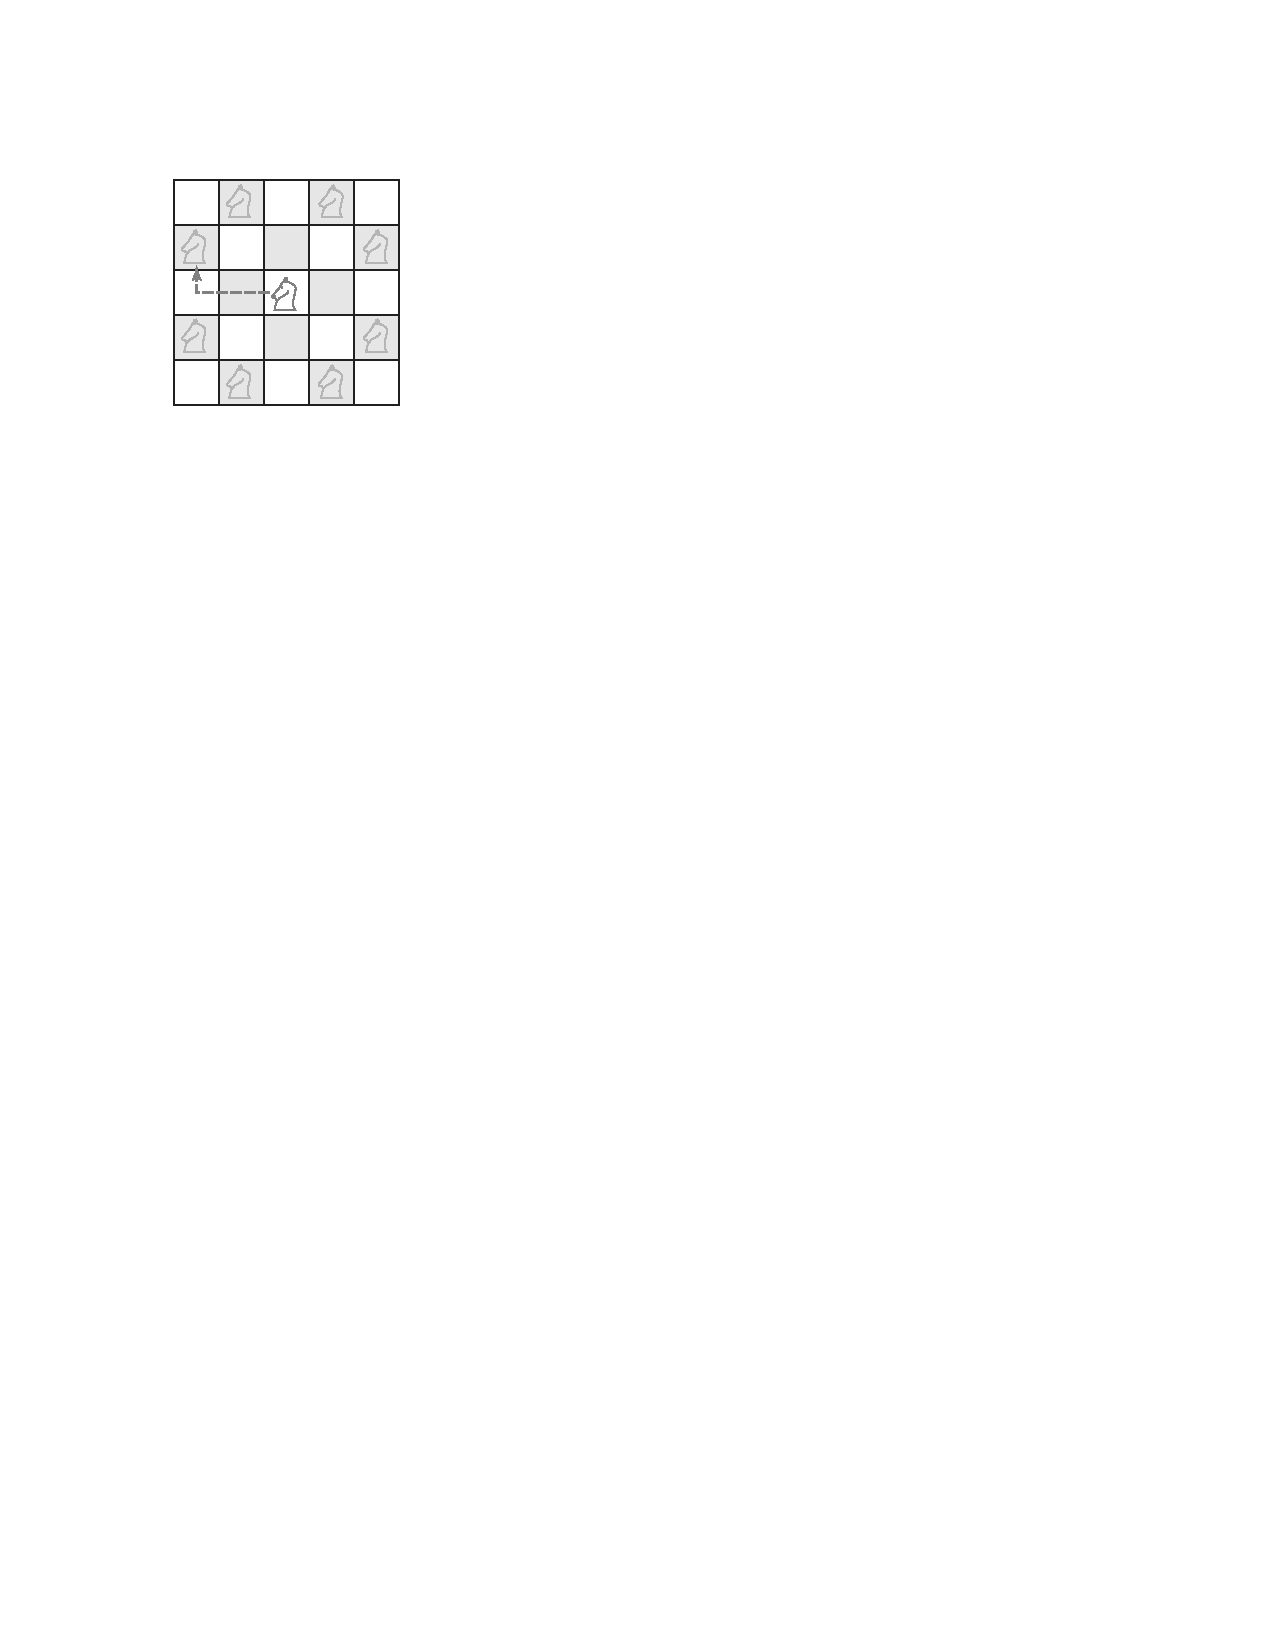
\includegraphics[width=\linewidth]{Images/Capitulo8/Chess.pdf}}
    \sideFigure[\label{fig:ajedreztab2}]{\centering
    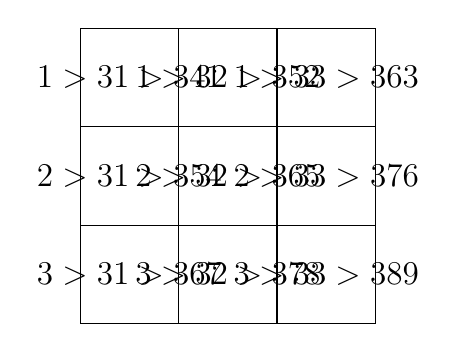
\begin{tikzpicture}
        \def\n{3}
        \def\m{3}
        \def\s{1.25cm}
        \draw grid[step=\s] (\n*\s, \m*\s);
        \foreach[evaluate] \x in {1,...,\n} {
            \foreach[evaluate={
                \zt = int(\x + \n*min(\y-1,\m+\y));
                \zb = int(\x + (\n-2)*min(\y-1,\m+\y)+3);
                }] \y in {1,...,\m} {
                \node[font=\large] at ({\s*(0.5+(\x-1))},{\s*(\m+0.5-\y)}) {$\ifthenelse{\y>3}{\ifthenelse{\x>3}{\zb}}{\zt}$};
                }
            };
    \end{tikzpicture}
    }
    \sideFigure[\label{fig:ajedreztab3}]{\centering
    \begin{tikzpicture}[font=\small]
        \def\dist{1.75cm}
        %%%%% COORDENADAS %%%%%
        \coordinate (P1) {};
        \coordinate[right=\dist of P1] (P2) {};
        \coordinate[right=\dist of P2] (P3) {};
        \coordinate[below=\dist of P3] (P6) {};
        \coordinate[left=\dist of P6] (P5) {};
        \coordinate[left=\dist of P5] (P4) {};
        \coordinate[below=\dist of P4] (P7) {};
        \coordinate[right=\dist of P7] (P8) {};
        \coordinate[right=\dist of P8] (P9) {};
        %%%%% FLECHAS %%%%%
        \draw (P1) -- (P8) -- (P3) -- (P4) -- (P9) -- (P2) -- (P7) -- (P6) -- (P1);
        \draw[{Stealth[scale=1.25]}-{Stealth[scale=1.25]}] ($(P1)!.1!(P8)$) -- ($(P1)!.9!(P8)$);
        \draw[{Stealth[scale=1.25]}-{Stealth[scale=1.25]}] ($(P8)!.1!(P3)$) -- ($(P8)!.9!(P3)$);
        \draw[{Stealth[scale=1.25]}-{Stealth[scale=1.25]}] ($(P3)!.1!(P4)$) -- ($(P3)!.9!(P4)$);
        \draw[{Stealth[scale=1.25]}-{Stealth[scale=1.25]}] ($(P4)!.1!(P9)$) -- ($(P4)!.9!(P9)$);
        \draw[{Stealth[scale=1.25]}-{Stealth[scale=1.25]}] ($(P9)!.1!(P2)$) -- ($(P9)!.9!(P2)$);
        \draw[{Stealth[scale=1.25]}-{Stealth[scale=1.25]}] ($(P2)!.1!(P7)$) -- ($(P2)!.9!(P7)$);
        \draw[{Stealth[scale=1.25]}-{Stealth[scale=1.25]}] ($(P7)!.1!(P6)$) -- ($(P7)!.9!(P6)$);
        \draw[{Stealth[scale=1.25]}-{Stealth[scale=1.25]}] ($(P6)!.1!(P1)$) -- ($(P6)!.9!(P1)$);
        %%%%% PUNTOS %%%%%
        \filldraw (P1) circle (1.75pt) node[above,minimum height=2em] {$1$};
        \filldraw (P2) circle (1.75pt) node[above,minimum height=2em] {$2$};
        \filldraw (P3) circle (1.75pt) node[above,minimum height=2em] {$3$};
        \filldraw (P4) circle (1.75pt) node[left,minimum width=2em] {$4$};
        \filldraw (P5) circle (1.75pt) node[above,minimum height=2em] {$5$};
        \filldraw (P6) circle (1.75pt) node[right,minimum width=2em] {$6$};
        \filldraw (P7) circle (1.75pt) node[below,minimum height=2em] {$7$};
        \filldraw (P8) circle (1.75pt) node[below,minimum height=2em] {$8$};
        \filldraw (P9) circle (1.75pt) node[below,minimum height=2em] {$9$};
    \end{tikzpicture}
    }
    \sideFigure[\label{fig:ajedreztab4}]{\centering
    \begin{tikzpicture}[font=\small, every node/.style={minimum size=2em}]
        \def\radius{2}
        %%%%% COORDENADAS %%%%%%
        \coordinate (O) {};
        \coordinate (P4) at ($(O) +(0*180:\radius)$) {};
        \coordinate (P3) at ($(O) +(0.25*180:\radius)$) {};
        \coordinate (P8) at ($(O) +(0.5*180:\radius)$) {};
        \coordinate (P1) at ($(O) +(0.75*180:\radius)$) {};
        \coordinate (P6) at ($(O) +(1*180:\radius)$) {};
        \coordinate (P7) at ($(O) +(1.25*180:\radius)$) {};
        \coordinate (P2) at ($(O) +(1.5*180:\radius)$) {};
        \coordinate (P9) at ($(O) +(1.75*180:\radius)$) {};
        %%%%% FLECHAS %%%%%
        \foreach \i in {0,1,2,...,7} {
        \draw[
            decoration={
                markings, mark=at position 0.0375+0.125*\i with {\arrow[>={Stealth[scale=1.25]}]{<}}
            },
            postaction={decorate}
        ] (O) circle (\radius);
        \draw[
            decoration={
                markings, mark=at position 0.1+0.125*\i with {\arrow[>={Stealth[scale=1.25]}]{>}}
            },
            postaction={decorate}
        ] (O) circle (\radius);
        }
        %%%%% PUNTOS %%%%%
        \filldraw (O) circle (1.75pt) node[above] {$5$};
        \filldraw (P4) circle (1.75pt) node[right] {$4$};
        \filldraw (P3) circle (1.75pt) node[right,yshift=0.1cm] {$3$};
        \filldraw (P8) circle (1.75pt) node[above] {$8$};
        \filldraw (P1) circle (1.75pt) node[left,yshift=0.1cm] {$1$};
        \filldraw (P6) circle (1.75pt) node[left,yshift=-0.1cm] {$6$};
        \filldraw (P7) circle (1.75pt) node[left,yshift=-0.1cm] {$7$};
        \filldraw (P2) circle (1.75pt) node[below] {$2$};
        \filldraw (P9) circle (1.75pt) node[right,yshift=-0.1cm] {$9$};
    \end{tikzpicture}
    }
    \noindent una dinámica única. Además, el hijo mayor ($A$) tiene la capacidad de influir en el hijo menor ($B$). Finalmente, el hijo menor ($B$) puede ejercer influencia sobre la madre ($M$). Podemos modelar este patrón de influencia familiar con un grafo dirigido cuyos vértices son los cinco miembros de la familia. Si el miembro de la familia $A$ influye en el miembro de la familia $B$, escribimos $A \rightarrow B$. La figura \ref{fig:grapfam} es el grafo dirigido resultante, donde hemos utilizado las anteriores designaciones para los cinco miembros de la familia. La matriz de vértices de este grafo dirigido es\\
    \begin{nscenter}
        \begin{tikzpicture}
            \node (A) at (0,0) {$\begin{bmatrix} 0 & 0 & 1 & 1 & 0 \\ 0 & 0 & 0 & 1 & 1 \\ 0 & 1 & 0 & 0 & 0 \\ 0 & 0 & 0 & 0 & 1 \\ 1 & 0 & 0 & 0 & 0 \end{bmatrix}$};
            \node[black!90!white, xshift=-1cm, yshift=0.1cm] at (A.north) {$M$};
            \node[black!90!white, xshift=-0.5cm, yshift=0.1cm] at (A.north) {$P$};
            \node[black!90!white, yshift=0.1cm] at (A.north) {$H$};
            \node[black!90!white, xshift=0.5cm, yshift=0.1cm] at (A.north) {$A$};
            \node[black!90!white, xshift=1cm, yshift=0.1cm] at (A.north) {$B$};
            \node[black!90!white, yshift=0.85cm, xshift=-0.1cm] at (A.west) {$M$};
            \node[black!90!white, yshift=0.47cm, xshift=-0.1cm] at (A.west) {$P$};
            \node[black!90!white, yshift=0.05cm, xshift=-0.1cm] at (A.west) {$H$};
            \node[black!90!white, yshift=-0.35cm, xshift=-0.1cm] at (A.west) {$A$};
            \node[black!90!white, yshift=-0.8cm, xshift=-0.1cm] at (A.west) {$B$};
        \end{tikzpicture}
    \end{nscenter}
\end{example}

\begin{example}
    En ajedrez, el caballo se mueve en un patrón en forma de “L” sobre el tablero. Para el tablero en la figura \ref{fig:ajedreztab}, puede moverse horizontalmente dos casillas y luego verticalmente una casilla, o puede moverse verticalmente dos casillas y luego horizontalmente una casilla. Así, desde la casilla central en la figura, el caballo puede moverse a cualquiera de las ocho casillas sombreadas marcadas. Supongamos que el caballo está restringido a las nueve casillas numeradas en la figura \ref{fig:ajedreztab2}. Si con $i \to j$ se quiere decir que el caballo puede moverse de la casilla $i$ a la casilla $j$, el grafo dirigido en la figura \ref{fig:ajedreztab3} ilustra todos los movimientos posibles que el caballo puede realizar entre estas nueve casillas. En la figura \ref{fig:ajedreztab4} hemos “desenredado” la figura \ref{fig:ajedreztab3} para hacer más claro el patrón de movimientos posibles. La matriz de vértices de este grafo dirigido es
    $$M = \begin{bmatrix}
        0 & 0 & 0 & 0 & 0 & 1 & 0 & 1 & 0 \\
        0 & 0 & 0 & 0 & 0 & 0 & 1 & 0 & 1 \\
        0 & 0 & 0 & 1 & 0 & 0 & 0 & 1 & 0 \\
        0 & 0 & 1 & 0 & 0 & 0 & 0 & 0 & 1 \\
        0 & 0 & 0 & 0 & 0 & 0 & 0 & 0 & 0 \\
        1 & 0 & 0 & 0 & 0 & 0 & 1 & 0 & 0 \\
        0 & 1 & 0 & 0 & 0 & 1 & 0 & 0 & 0 \\
        1 & 0 & 1 & 0 & 0 & 0 & 0 & 0 & 0 \\
        0 & 1 & 0 & 1 & 0 & 0 & 0 & 0 & 0 
    \end{bmatrix}$$
\end{example}

En el ejemplo \ref{exam:graf1}, el padre no puede influir directamente a la madre; es decir, $P \to M$ no es cierto. Sin embargo, puede influir en el hijo menor, quien a su vez puede influir en la madre. Esto se escribe como $P \to B \to M$ y se denomina una conexión de $2$ pasos de $P$ a $M$. De manera similar, $M \to H$ es una conexión de $1$ paso, mientras que $P \to A \to B \to M$ es una conexión de $3$ pasos, y así sucesivamente.

Consideremos ahora una técnica para determinar el número de todas las posibles conexiones de $r$ pasos ($r = 1, 2, \dots$) desde un vértice $P_i$ hasta otro vértice $P_j$ en un grafo dirigido arbitrario (esto incluye el caso en que $P_i$ y $P_j$ sean el mismo vértice). El número de conexiones de $1$ paso desde $P_i$ hasta $P_j$ es simplemente $m_{ij}$. Es decir, hay cero o una conexión de $1$ paso desde $P_i$ hasta $P_j$, dependiendo de si $m_{ij}$ es cero o uno. Para el número de conexiones de $2$ pasos, consideramos el cuadrado de la matriz de vértices. Si designamos $m_{ij}^{(2)}$ como el elemento $(i, j)$-ésimo de $M^2$, tenemos que
\begin{equation}
    m_{ij}^{(2)} = m_{i1}m_{ij} + m_{i2}m_{2j} + \cdots + m_{in}m_{nj} \label{eq:grafos1}
\end{equation}
Ahora bien, si $m_{i1} = m_{1j} = 1$, hay una conexión de $2$ pasos $P_i \to P_1 \to P_j$ desde $P_i$ hasta $P_j$. Sin embargo, si $m_{i1}$ o $m_{1j}$ es cero, dicha conexión de $2$ pasos no es posible. Por lo tanto, $P_i \to P_1 \to P_j$ es una conexión de $2$ pasos solo si $m_{i1}m_{1j} = 1$. De manera similar, para cualquier $k = 1, 2, \dots, n$, $P_i \to P_k \to P_j$ es una conexión de $2$ pasos desde $P_i$ hasta $P_j$ solo si el término $m_{ik}m_{kj}$ en el lado derecho de \eqref{eq:grafos1} es uno; de lo contrario, el término es cero. Así, el lado derecho de \eqref{eq:grafos1} representa el número total de conexiones de $2$ pasos desde $P_i$ hasta $P_j$.

Un razonamiento similar se puede aplicar para encontrar el número de conexiones de $3$, $4$, $\dots$, $r$ pasos desde $P_i$ hasta $P_j$. En general, obtenemos el siguiente resultado.

\begin{theorem}\label{theo:rconexiones}
    Sea $M$ la matriz de vértices de un grafo dirigido y sea $m^{(r)}_{ij}$ el elemento $(i, j)$-ésimo de $M^r$. Entonces, $m^{(r)}_{ij}$ es igual al número de conexiones de $r$ pasos desde $P_i$ hasta $P_j$.
\end{theorem}

\begin{example}
    \sideFigure[\label{fig:examgrafoss3}]{\centering
    \begin{tikzpicture}
        %%%%% COORDENADAS %%%%%
        \coordinate (P1) {};
        \coordinate[above right=3cm and 3cm of P1] (P2) {};
        \coordinate[below right=3.1cm and 1.4cm of P2] (P3) {};
        \coordinate[below left=2.5cm and 2.9cm of P3] (P4) {};
        %%%%% PUNTOS %%%%%
        \filldraw (P1) circle (1.75pt) node[left] {$P_1$};
        \filldraw (P2) circle (1.75pt) node[above] {$P_2$};
        \filldraw (P3) circle (1.75pt) node[right] {$P_3$};
        \filldraw (P4) circle (1.75pt) node[below] {$P_4$};
        %%%%% FLECHAS %%%%%
        \draw (P1) -- (P2) -- (P3) -- (P4);
        \draw[name path=P1--P3] (P1) -- (P3);
        \draw[name path=P2--P4] (P2) -- (P4);
        \path[name intersections={of=P1--P3 and P2--P4,by=P}];
        \draw[{Stealth[scale=1.25]}-{Stealth[scale=1.25]}] ($(P1)!.25!(P2)$) -- ($(P1)!.75!(P2)$);
        \draw[-{Stealth[scale=1.25]}] (P2) -- ($(P2)!.5!(P3)$);
        \draw[{Stealth[scale=1.25]}-{Stealth[scale=1.25]}] ($(P3)!.25!(P4)$) -- ($(P3)!.75!(P4)$);
        \draw[-{Stealth[scale=1.25]}] (P) -- ($(P)!.5!(P1)$);
        \draw[-{Stealth[scale=1.25]}] (P) -- ($(P)!.5!(P2)$);
        \draw[-{Stealth[scale=1.25]}] (P) -- ($(P)!.5!(P3)$);
    \end{tikzpicture}
    }
    La figura \ref{fig:examgrafoss3} es el mapa de rutas de una pequeña aerolínea que opera en las cuatro ciudades $P_1$, $P_2$, $P_3$, y $P_4$. Como un grafo dirigido, su matriz de vértices es
    $$M = \begin{bmatrix}
        0 & 1 & 1 & 0 \\
        1 & 0 & 1 & 0 \\
        1 & 0 & 0 & 1 \\
        0 & 1 & 1 & 0
    \end{bmatrix}$$
    y además, tenemos que
    $$M^2 = \begin{bmatrix}
        2 & 0 & 1 & 1 \\
        1 & 1 & 1 & 1 \\
        0 & 2 & 2 & 0 \\
        2 & 0 & 1 & 1
    \end{bmatrix} \quad \text{ y } \quad M^3 = \begin{bmatrix}
        1 & 3 & 3 & 1 \\
        2 & 2 & 3 & 1 \\
        4 & 0 & 2 & 2 \\
        1 & 3 & 3 & 1
    \end{bmatrix}$$
    Si estamos interesados en las conexiones de la ciudad $P_4$ a la ciudad $P_3$, podemos usar el teorema \ref{theo:rconexiones} para encontrar su número. Dado que $m_{43} = 1$, hay una conexión de un paso; dado que $m_{43}^{(2)} = 1$, hay una conexión de dos pasos; y dado que $m_{43}^{(3)} = 3$, hay tres conexiones de tres pasos. Para verificar esto, en la figura \ref{fig:examgrafoss3} encontramos que
    \begin{align*}
        \text{Conexiones de un paso de } P_4 \text{ a } P_3:& & P_4 &\to P_3 \\
        \text{Conexiones de dos pasos de } P_4 \text{ a } P_3:& & P_4 &\to P_2 \to P_3 \\
        \text{Conexiones de tres pasos de } P_4 \text{ a } P_3:& & P_4 &\to P_3 \to P_4 \to P_3 \\
        & & P_4 &\to P_2 \to P_1 \to P_3 \\
        & & P_4 &\to P_3 \to P_1 \to P_3
    \end{align*}
\end{example}

\subsection*{Cliques}

En lenguaje cotidiano, una "clique" es un grupo de personas muy unido (usualmente de tres personas o más) que tiende a comunicarse entre sí y no tiene espacio para los extraños. En la teoría de grafos, este concepto se define de manera más precisa.

\begin{definition}
    Un subconjunto de un grafo dirigido se llama “clique” si cumple con las siguientes tres condiciones:
    \begin{enumerate}[label=\roman*)]
        \item El subconjunto contiene al menos tres vértices.
        \item Para cada par de vértices $P_i$ y $P_j$ en el subconjunto, se cumplen tanto $P_i \rightarrow P_j$ como $P_j \rightarrow P_i$.
        \item El subconjunto es lo más grande posible; es decir, no es posible agregar otro vértice al subconjunto y seguir cumpliendo la condición (ii).
    \end{enumerate}
\end{definition}

\newpage\noindent
Esta definición implica que una clique es un subconjunto máximo de vértices que están en perfecta “comunicación” entre sí. Por ejemplo, si los vértices representan ciudades y $P_i \rightarrow P_j$ indica que hay un vuelo directo entre la ciudad $P_i$ y la ciudad $P_j$, entonces dentro de una clique, cada par de ciudades tiene un vuelo directo en ambas direcciones.

\begin{definition}
    \sideFigure[\label{fig:examgrafoss3}]{\centering
    \begin{tikzpicture}
        %%%%% COORDENADAS %%%%%
        \coordinate (P1) {};
        \coordinate[above right=2cm and 1.25cm of P1] (P2) {};
        \coordinate[above left=2cm and 1.25cm of P2] (P3) {};
        \coordinate[below right=2cm and 3.5cm of P3] (P4) {};
        \coordinate[above left=4cm and 2cm of P4] (P5) {};
        \coordinate[below right=2cm and 2.5cm of P5] (P6) {};
        \coordinate[below left=3.5cm and 1.5cm of P6] (P7) {};
        %%%%% PUNTOS %%%%%
        \filldraw (P1) circle (1.75pt) node[below] {$P_1$};
        \filldraw (P2) circle (1.75pt) node[right,yshift=-0.2cm] {$P_2$};
        \filldraw (P3) circle (1.75pt) node[left] {$P_3$};
        \filldraw (P4) circle (1.75pt) node[right] {$P_4$};
        \filldraw (P5) circle (1.75pt) node[above] {$P_5$};
        \filldraw (P6) circle (1.75pt) node[right] {$P_6$};
        \filldraw (P7) circle (1.75pt) node[right] {$P_7$};
        %%%%% FLECHAS %%%%%
        \draw (P1) -- (P2) -- (P3) -- (P1) -- (P4) -- (P2) -- (P1) -- (P4) -- (P3) -- (P5) -- (P6) -- (P3) -- (P5) -- (P6) -- (P4) -- (P7);
        \draw[{Stealth[scale=1.25]}-{Stealth[scale=1.25]}] ($(P1)!.25!(P3)$) -- ($(P1)!.75!(P3)$);
        \draw[{Stealth[scale=1.25]}-{Stealth[scale=1.25]}] ($(P1)!.25!(P2)$) -- ($(P1)!.75!(P2)$);
        \draw[{Stealth[scale=1.25]}-{Stealth[scale=1.25]}] ($(P1)!.25!(P4)$) -- ($(P1)!.75!(P4)$);
        \draw[{Stealth[scale=1.25]}-{Stealth[scale=1.25]}] ($(P2)!.25!(P4)$) -- ($(P2)!.75!(P4)$);
        \draw[{Stealth[scale=1.25]}-{Stealth[scale=1.25]}] ($(P3)!.25!(P4)$) -- ($(P3)!.75!(P4)$);
        \draw[{Stealth[scale=1.25]}-{Stealth[scale=1.25]}] ($(P2)!.25!(P3)$) -- ($(P2)!.75!(P3)$);
        \draw[{Stealth[scale=1.25]}-{Stealth[scale=1.25]}] ($(P3)!.25!(P6)$) -- ($(P3)!.75!(P6)$);
        \draw[{Stealth[scale=1.25]}-{Stealth[scale=1.25]}] ($(P4)!.25!(P6)$) -- ($(P4)!.75!(P6)$);
        \draw[{Stealth[scale=1.25]}-{Stealth[scale=1.25]}] ($(P7)!.25!(P4)$) -- ($(P7)!.75!(P4)$);
        \draw[-{Stealth[scale=1.25]}] (P3) -- ($(P3)!.5!(P5)$);
        \draw[-{Stealth[scale=1.25]}] (P5) -- ($(P5)!.5!(P6)$);
    \end{tikzpicture}
    }
    El grafo dirigido ilustrado en la figura \ref{fig:examgrafoss3} (que podría representar el mapa de rutas de una aerolínea) tiene dos cliques:
    $$\{P_1, P_2, P_3, P_4\} \quad \text{ y } \quad \{P_3, P_4, P_6\}$$
    Este ejemplo muestra que un grafo dirigido puede contener varios cliques y que un vértice puede pertenecer a más de un clique simultáneamente.
\end{definition}

%\section{Juegos de estrategia}

%\section{Modelos económicos de Leontief}

%\section{Gestión forestal}

%\section{Gráficos por computadora}

%\section{Distribuciones de temperatura en equilibrio}

%\section{Tomografía computarizada}

%\section{Fractales}

%\section{Caos}

%\section{Criptografía}

%\section{Genética}

%\section{Cosecha de poblaciones de animales}

%\section{Motores de búsqueda en Internet}